%%%%%%%%%%%%%%%%%%%%%%%%%%%%%%%%%%%%%%%%%%%%%%%%%%%%%%%%
%%%%%%%%%%%%%%%%%%%%%%%%%%%%%%%%%%%%%%%%%%%%%%%%%%%%%%%%
\newpage
\part*{Árboles}
\setcounter{section}{0}

Una vez estudiada las estructuras de datos lineales como pilas y colas y con experiencia en recursión, estudiaremos el tipo de dato llamado Tree (árbol). Los árboles son empleados en muchas áreas de las Ciencias de la Computación, que se incluyen sistemas operativos, gráficos, sistemas de base de datos, y redes de computadoras. Las estructuras de datos Tree tiene mucho en común con su equivalente en botánica. Un tree tiene raíz, ramas y hojas. La principal diferencia radica en que la raíz se encuentra en la parte superior y las hojas en la parte inferior.

Conceptualmente, el árbol es una estructura de datos jerárquica que puede ser definida recursivamente como una colección de nodos, y cada nodo tiene un valor junto con una lista que referencia a un conjunto de nodos. Del mismo modo, los árboles tienen como restricción que no existen elementos duplicados y ningún elemento apunta a la raíz. Pueden existir árboles vacíos y conjuntos de árboles (llamados bosques).

Un ejemplo se puede ver a continuación:

\begin{figure}[htpb!]
  \begin{center}
    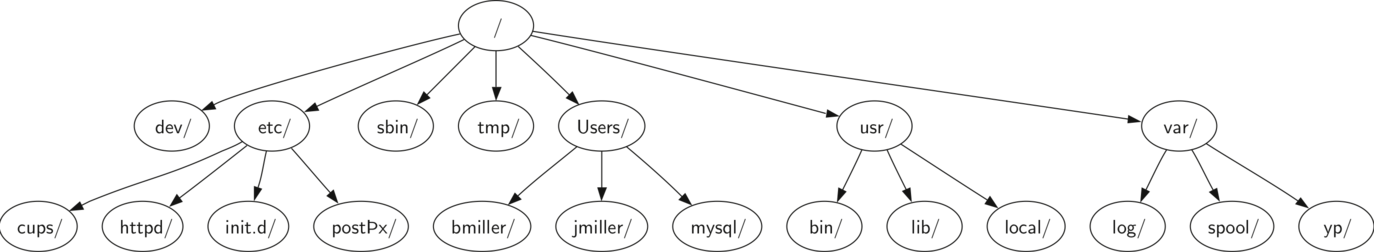
\includegraphics[width=1.0\textwidth]{images/extree1.png}
  \end{center}
  \caption{El árbol representa el sistema de archivos en Unix. En un sistema de archivos existen archivos y directorios como una estructura de árbol.}
  \label{fig:extree1}
\end{figure}

Nótese que empezando desde la raíz, se puede recorrer hasta la parte inferior del árbol en un único camino. Igualmente, se puede ver que todos los hijos de un nodo son independientes de los hijos de otro nodo. Así, cada nodo de la parte inferior (nodo hoja) es único, es decir, existe un solo camino para llegar a éste.

Como es sabido, es posible mover un directorio completo de un lugar del sistema de archivos a otros. Cuando se realiza este proceso, todos los hijos asociados q dicho nodo se moverán (a este conjunto de nodos se denomina sub-árbol). Por ejemplo, es posible mover el sub-arbol que empieza en /etc/ (quitarlo del nodo /) y colocarlo por debajo de /usr. Así, la ruta de acceso a httpd cambiará, quedando /usr/etc/http/ sin afectar el contenido o a cualquier directorio hijo de http.

Otro ejemplo basado en un sistema de árbol es una página Web escrita en HTML. Para el siguiente código en HTML:

\begin{lstlisting}[upquote=true, language=html]
<html xmlns="http://www.w3.org/1999/xhtml"
      xml:lang="en" lang="en">
<head>
    <meta http-equiv="Content-Type"
          content="text/html; charset=utf-8" />
    <title>Premio Nobel</title>
</head>
<body>
<h1>Los candidatos al premio son:</h1>
<ul>
    <li>Homer J. Simpson</li>
    <li>Peter Griffin</li>
</ul>
<h2><a href="http://www.fakepage.org/voting">Consultar las votaciones</a><h2>
</body>
</html>
\end{lstlisting}

Su árbol asociado se muestra en la Fig. \ref{fig:treeHTML}.

\begin{figure}[htpb!]
  \begin{center}
    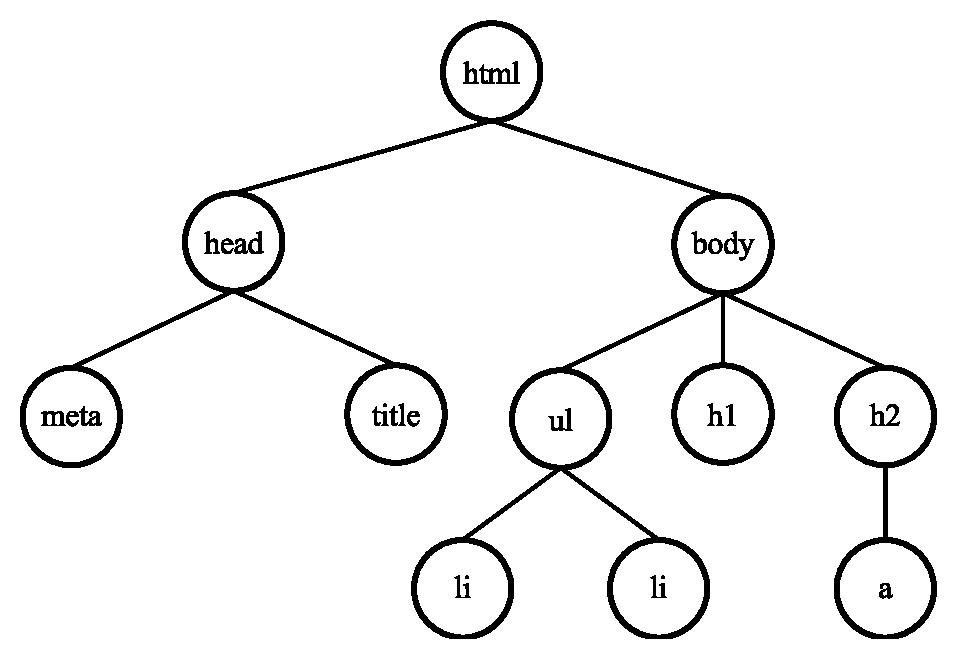
\includegraphics[width=0.5\textwidth]{images/treeHTML.eps}
  \end{center}
  \caption{Representación en forma de árbol del ejemplo de código en HTML.}
  \label{fig:treeHTML}
\end{figure}

%%%%%%%%%%%%%%%%%%%%%%%%%%%%%%%%%%%%%%%%%%%%%%%%%%%%%%%%
\section{Definiciones}

Formalmente, un árbol es un grafo conexo acíclico cuyos nodos se relacionan mediante una jerarquía.

En su implementación, un árbol de tipo $T$ es una estructura homogénea producto de la concatenación de un elemento de tipo $T$ junto con un número finito de árboles disjuntos (sub-árboles). Una forma particular de un árbol es una estructura vacía. Un árbol puede ser representado por una estructura estática (arreglos/registros/clases) ó dinámica (apuntadores/listas).

De forma recursiva, un árbol es una colección de nodos ${T_1, T_2,\dots, T_k}$ del mismo tipo tal que:
\begin{itemize}
\item Si $k == 0$, entonces el árbol es vacío
\item Si $k > 0$, entonces existe un nodo especial llamado raíz (generalmente el primero de la definición, i.e. $T_1$) y los demás nodos forman parte de $n \ge 0$ conjuntos disjuntos que a su vez son árboles. Estos árboles se denominan sub-árboles del nodo raíz
\end{itemize}

\textbf{Conceptos asociados en la estructura Tree}
\begin{description}
\item[Nodo -] Es la parte fundamental del árbol. Es posible que contenga un identificador (llamado key) e información adicional (payload)
\item[Enlace– ] Algunas veces llamadas ramas, es otra parte fundamental del árbol, un enlace conecta dos nodos y muestra la relación que existe entre éstos. Cada nodo, con excepción de la raíz, está conectado con exactamente un enlace entrante desde otro nodo. Cada nodo puede tener muchos enlaces salientes
\item[Raíz –] La raíz de un árbol es el único nodo del árbol que no tiene enlaces entrantes. Por ejemplo, el nodo \textit{html}
\item[Hijos –] El conjunto de nodos $c$ que tienen enlaces entrantes desde un mismo nodo $n$ se denominan hijos de $n$. Por ejemplo, los nodos \textit{meta} y \textit{title} son hijos del nodo \textit{head}.
\item[Padre –] El concepto inverso a Hijo.
\item[Hermanos –] Nodos con el mismo padre.
\item[Camino –] Un camino es una lista ordenada de nodos conectadas por enlaces. Por ejemplo \textit{html} $\to$ \textit{body} $\to$ \textit{h1}
\item[Longitud de un camino –] Es el número de veces que se debe aplicar la relación padre-hijos entre dos nodos que forman un camino
\item[Descendiente –] Un nodo alcanzable por un proceso repetitivo empleando los enlaces desde padres a sus hijos (un camino).
\item[Ancestro -] A veces llamado antecesor, es un nodo alcanzable por un proceso repetitivo empleando los enlaces desde los hijos a sus padres (un camino)
\item[Sub-árbol –] Un subárbol es un conjunto de nodos y enlaces formados por un padre y todos los descendientes de ese padre.
\item[Nodo Hoja –] También llamado nodo terminal ó externo. Es un nodo que no tiene hijos.
\item[Nodo Interno –] También llamado nodo no-terminal. Es un nodo con al menos un hijo (no es hoja).
\item[Grado –] Es el número de sub-árboles de un nodo.
\item[Grado de un árbol –] Es el máximo grado de todos los nodos del árbol, i.e. la cantidad máxima de hijos que soporta cada nodo
\item[Nivel –] Es la longitud del camino desde la raíz hasta un nodo. Si un árbol solo contiene la raíz, su nivel es 0.
\item[Altura –] La altura de un árbol se cuenta como el número de enlaces desde el nodo raíz hasta la hoja más lejana, es decir, el máximo nivel de cualquier nodo en el árbol.
\item[Profundidad –] La longitud máxima del camino desde un nodo a cualquier de sus descendientes.
\item[Peso –] El peso de un árbol se refiere al número de nodos que contiene el árbol.
\item[Bosque –] Un bosque es un conjunto de $n \ge 0$ árboles disjuntos
\end{description}

%%%%%%%%%%%%%%%%%%%%%%%%%%%%%%%%%%%%%%%%%%%%%%%%%%%%%%%%
\section{General Tree}

Una estructura General Tree o árbol general $T$ es un conjunto finito de uno o más nodos donde existe un nodo designado $r$ llamado raíz de $T$, y los nodos restantes son particionados en $n \ge 0$ conjuntos disjuntos $T_1, T_2, \dots, T_k$ donde cada uno es un árbol y cuyas raíces $r_1, r_2, \dots, r_k$ son hijos de $r$. En la Fig. \ref{fig:gentree} se muestra un ejemplo de árbol general de altura 3, grado 4, peso 9, con nodo raíz 2, conteniendo 6 hojas/nodos externos/nodos terminales y 3 nodos internos/no-terminales.

\begin{figure}[htpb!]
  \begin{center}
    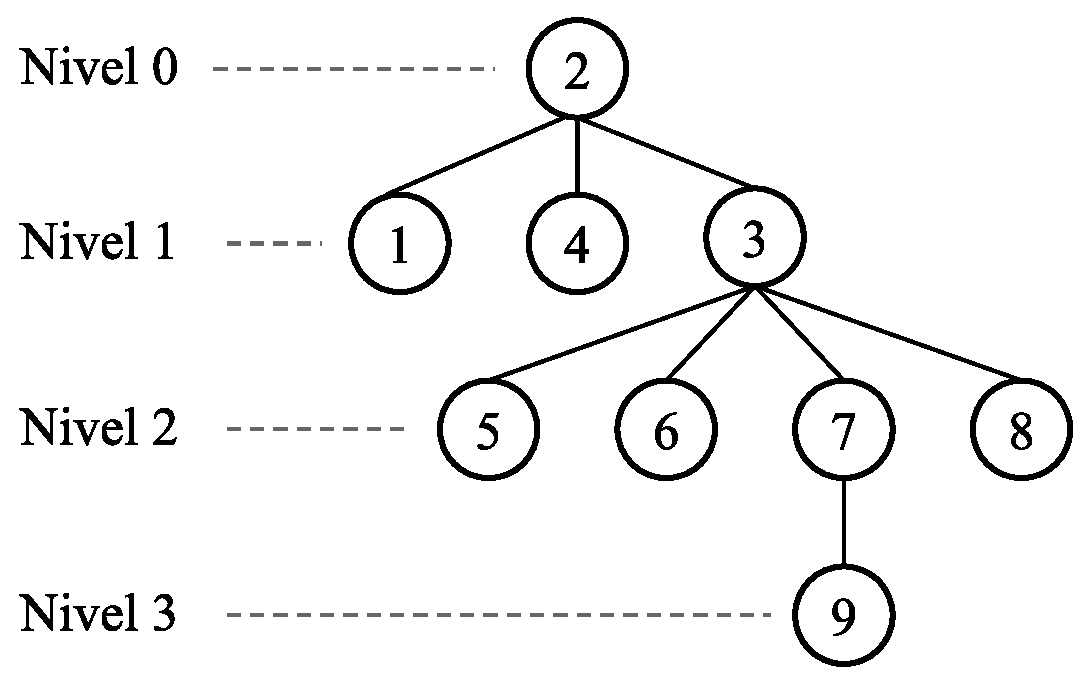
\includegraphics[width=0.55\textwidth]{images/gentree.eps}
  \end{center}
  \caption{Ejemplo de un árbol general de grado 4 (cuaternario) y altura 3.}
  \label{fig:gentree}
\end{figure}

Nótese que el árbol general de grado $g$ puede desde $0$ hijos (nodo terminal) a $g$ hijos (nodo no-terminal) para cada nodo.

%%%%%%%%%%%%%%%%%%%%%%%%%%%
\subsection{Especificación}

Se muestra a continuación la especificación de la clase GenTree que representa a un árbol general.

\begin{lstlisting}[upquote=true, language=pseudo]
class GenTree <T>
public:
  Constructor GenTree()			//crea un árbol vacío
  Destructor GenTree()			//destruye el árbol 
  function GetRoot () : Node	//retorna el nodo correspondiente a la raíz
  function GetChild (Node idNode) : Node	//retorna el nodo del 1er hijo de idNode (según convención, el más a la izq)
  function GetRBrother(Node idNode) : Node	//retorna la raíz del 1er sub-árbol a la der de idNode con el mismo padre
  function ExistRBrother(Node idNode) : Boolean	//indica si tiene hermano derecho
  function GetValue(Node idNode) : T	//retorna el contenido del nodo idNode
  function GetParent(Node idNode) : Node	//retorna el padre de idNode
  function isLeaf(Node idNode) : Boolean	//retorna verdad/falso si idNode es hoja
  function isEmpty() : Boolean	//retorna verdad/falso si el árbol no contiene nodos
  function Insert(Node idNode)	//inserta el nodo idNode al árbol (no se especifica dónde)
  function Delete(Node idNode)	//elimina el nodo idNode del árbol
end
\end{lstlisting}

Un ejemplo para el cálculo del nivel en un GenTree es como sigue:

\begin{lstlisting}[upquote=true, language=pseudo]
function Level(Node<T> idNode) : Integer
  Integer iLevel = 0
  Node<T> nTemp = idNode
  while nTemp  != EMPTY do
    nTemp = GetParent(nTemp)
    iLevel = iLevel + 1
  end
  return iLevel
end
\end{lstlisting}

Dado que no se conoce la implementación aún del árbol general, se emplea idNode el cual representa un identificador de un nodo del árbol. La idea es algoritmo es ir subiendo hasta la raíz (usando el padre) e ir contando hasta que no se pueda más (nodo raíz). Nótese que si se invoca la función con el nodo más "profundo" (el de mayor nivel) es equivalente a la altura del árbol.

%%%%%%%%%%%%%%%%%%%%%%%%%%%
\subsection{Implementación}

Para la implementación del tipo GenTree se requiere de una estructura tipo Node que almacene el valor de la información del árbol (el tipo T) e información de los hijos de dicho nodo. Es importante destacar que cada nodo representa a un árbol, o subárbol, por lo que tiene 0 o más hijos. Una primera implementación se puede definir como un arreglo de punteros al tipo Node.

\begin{lstlisting}[upquote=true, language=pseudo]
class Node<T>
public:
  T tInfo
  Array aChild of Node<T>* [1..N]
end

class GenTree<T>
private:
  Node<T>* pRoot
public:
  ... //the public functions
end
\end{lstlisting}

En dicha implementación, se requiere definir el número máximo de hijos que puede tener un nodo. Es decir, si se conoce el grado del árbol, entonces el número máximo de dicho árbol corresponde con el grado del árbol. Sin embargo, es posible que en un momento dado una gran parte de los nodos tenga un número de nodos menor al grado del árbol, implicando que se desperdicie memoria en dicha implementación. Así, una mejor implementación requiere solo crear/reservar espacio en memoria de los nodos que son creados. Para ello, una implementación en donde los hijos de un nodo se construyen como una lista basada en apuntadores resulta eficiente. A continuación se muestra un ejemplo de ello.

\begin{lstlisting}[upquote=true, language=pseudo]
class Node<T>
public:
  T tInfo
  List<T> L
end

class GenTree<T>
private:
  Node<T>* pRoot
public:
  ... //the public functions
end
\end{lstlisting}

%%%%%%%%%%%%%%%%%%%%%%%%%%%
\subsection{Recorridos}

El proceso de recorrido de un árbol consiste en visitar/recorrer/consultar o realizar una acción en cada nodo tal que no modifique la estructura del árbol (e.g. imprimir, contar, comparar). Esta visita se realiza bajo cierto orden y la acción se efectúa una sola vez por nodo. Básicamente se pueden definir dos recorridos para árboles generales: preorden o postorden.

El recorrido en preorden consiste en recorrer primeramente el nodo raíz, y luego los nodos que contienen a los hijos desde el nodo más a la izquierda hasta el nodo más a la derecha. El recorrido postorden primero recorre los nodos hijos de derecha a izquierda y luego el nodo raíz.

En el ejemplo mostrado en la Fig. \ref{fig:gentree} sus respectivos recorridos son:

Preorden: 2, 1, 4, 3, 5, 6, 7, 9, 8

Postorden: 1, 4, 5, 6, 9, 7, 8, 3, 2

%%%%%%%%%%%%%%%%%%%%%%%%%%%%%%%%%%%%%%%%%%%%%%%%%%%%%%%%
\section{Binary Tree - BT}

Es posible representar diversos comportamientos empleando decisiones de aceptar/rechazar, si/no, fuera/dentro, etc. En Ciencias de la Computación, se suele emplear estructuras de datos que permitan manejar dichos comportamientos para solucionar diversos problemas. Por ejemplo, el lanzamiento de una moneda (i.e. moneda ideal) solo tiene dos posibilidades: cara (H) o sello (T). Así, el evento de lanzamiento de una moneda se puede representar como un árbol de decisión. Por ejemplo el lanzamiento de una moneda se puede graficar como se muestra en la Fig. \ref{fig:tree3coins}

\begin{figure}[htpb!]
  \begin{center}
    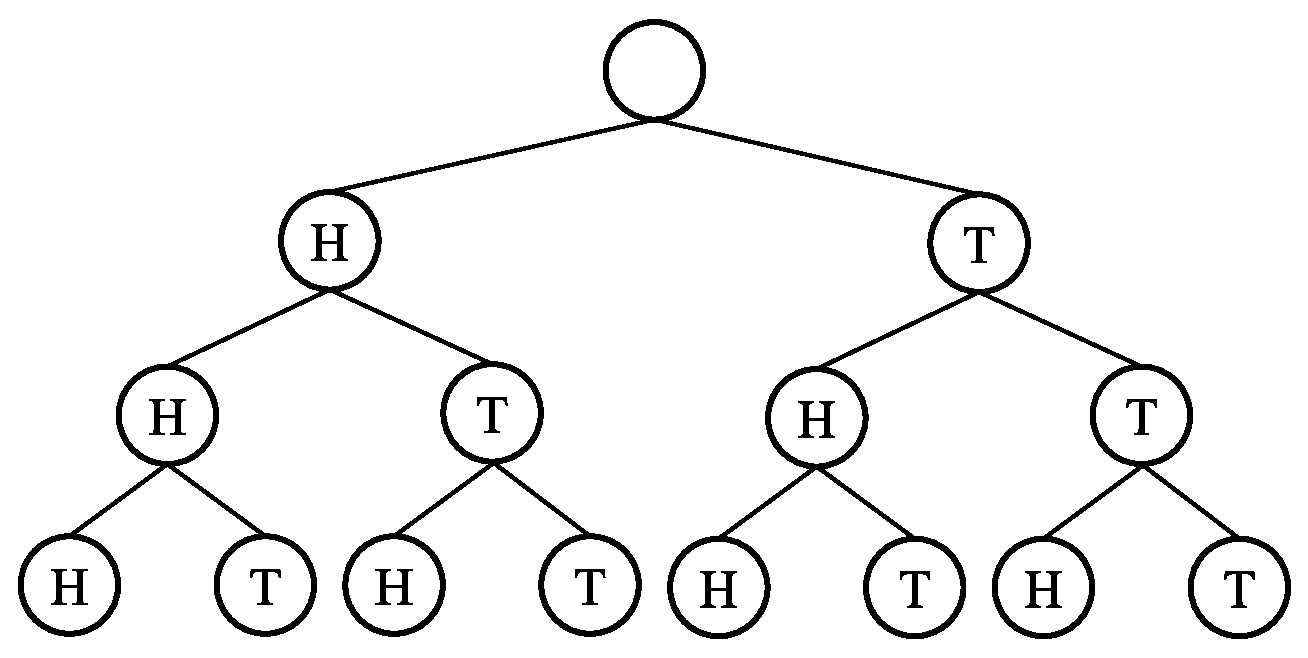
\includegraphics[width=0.4\textwidth]{images/gen3coins.eps}
  \end{center}
  \caption{Ejemplo del lanzamiento de una moneda 3 veces seguidas.}
  \label{fig:tree3coins}
\end{figure}

Por cada lanzamiento es posible obtener H o T, entonces partiendo desde la raíz se muestran las 8 posibles combinaciones (de izquierda a derecha): HHT, HHT, HTH, HTT, THH, THT, TTH y TTT.

%%%%%%%%%%%%%%%%%%%%%%%%%%%%%%
\subsection{Definiciones}

En la teoría de árboles, un árbol es llamado k-ario si cada nodo contiene como máximo k hijos. Un caso particular es el árbol binario donde $k=2$. Si todos los nodos del árbol, a excepción de las hojas, posee exactamente $k$ hijos entonces dicho árbol es completo.

%%%%%%%%%%%%%%%%%%%%%%%%%%%%%%
\subsection{Recorridos}

\begin{lstlisting}[upquote=true, language=pseudo]
void Preorder (IdNode root)
  if root == EMPTY then
    Visit (root)
    Preorder (Left(root))
    Preorder (Right(root))
  end
end
\end{lstlisting}

\begin{lstlisting}[upquote=true, language=pseudo]
void Inorder (IdNode root)
  if root == EMPTY then
    Inorder (Left(root))
    Visit (root)
    Inorder (Right(root))
  end
end
\end{lstlisting}


\begin{lstlisting}[upquote=true, language=pseudo]
void Postorder (IdNode root)
  if root == EMPTY then
    Postorder (Left(root))
    Postorder (Right(root))
    Visit (root)
  end
end
\end{lstlisting}

En la Fig. \ref{fig:bintreeExpresion} se observa un ejemplo de árbol binario para representar una expresión aritmética. Al ejecutar los 3 recorridos sobre el árbol queda:

Preorder: + - A * B C D (expresión prefija) \\
Inorder: A - B * C + D (expresión infija) \\
Postorder: + - A * B C D (expresión postfija) \\

\begin{figure}[htpb!]
  \begin{center}
    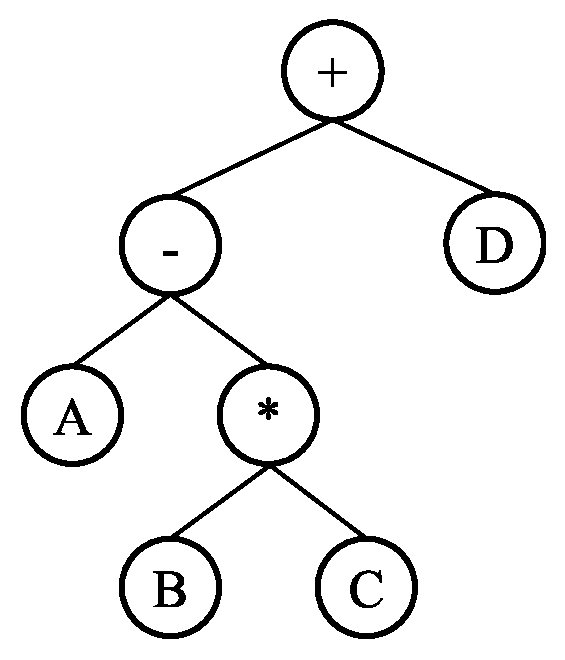
\includegraphics[width=0.25\textwidth]{images/bintreeExpresion.eps}
  \end{center}
  \caption{Ejemplo de la representación de un BST para almacenar expresiones aritméticas.}
  \label{fig:bintreeExpresion}
\end{figure}



%%%%%%%%%%%%%%%%%%%%%%%%%%%%%%
\subsection{Implementación}

\paragraph{Implementación basada en arreglos}

La implementación de un BST empleando arreglos debe conocer el número máximo de nodos o estimarlo (estática o dinámica) tal que en cada posición se almacene un nodo. La idea es almacenar los hijos izquierdo y derecho, en ese orden, de un nodo $k$ en las posiciones $2 \times k + 1$ y $2 \times k + 2$ respectivamente. En la Fig. \ref{fig:vectorbinTree} se muestra un ejemplo de la implementación basada en arreglos.

\begin{figure}[htpb!]
  \begin{center}
    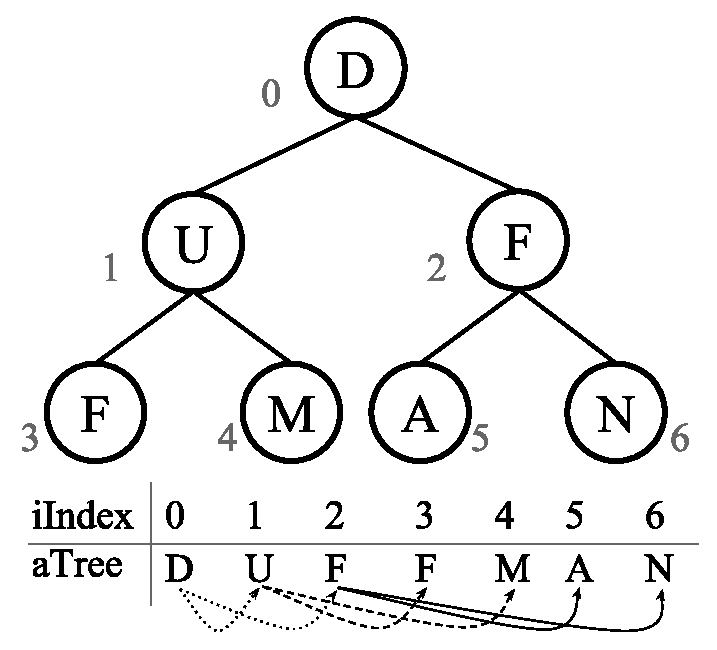
\includegraphics[width=0.4\textwidth]{images/vectorbinTree.eps}
  \end{center}
  \caption{Representación de un árbol completo del tipo Char almacenado dentro de un arreglo.}
  \label{fig:vectorbinTree}
\end{figure}

El árbol $aTree$ tiene 7 nodos con de altura 2, y la variable iIndex representa su posición a ser almacenada en dicho arreglo. Nótese la numeración es de arriba hacia abajo y de izquierda a derecha.

Esta representación es muy buena para árboles completos, pero muy mala para árboles degenerados.

\paragraph{Implementación basada en apuntadores}

La idea detrás de la implementación de un árbol binario basado en apuntadores es la creación de un nodo que contenga un puntero al hijo izquierdo, al hijo derecho y a la información/datos a almacenar. El puntero a la raíz apunta al nodo más arriba en el árbol. Los punteros derecho e izquierdo apuntan recursivamente a cada subárbol de cada lado, tal como se muestra en la figura \ref{fig:BTPointer}. Se puede observar que en la raíz está el valor de 500 y como hijo derecho al subárbol cuyo nodo raíz contiene al valor 569, y como hijo izquierdo el nodo (subárbol) que contiene el valor de 300. Los nodos hoja tienen los punteros a ambos hijos a nulo.

\begin{figure}[htpb!]
  \begin{center}
    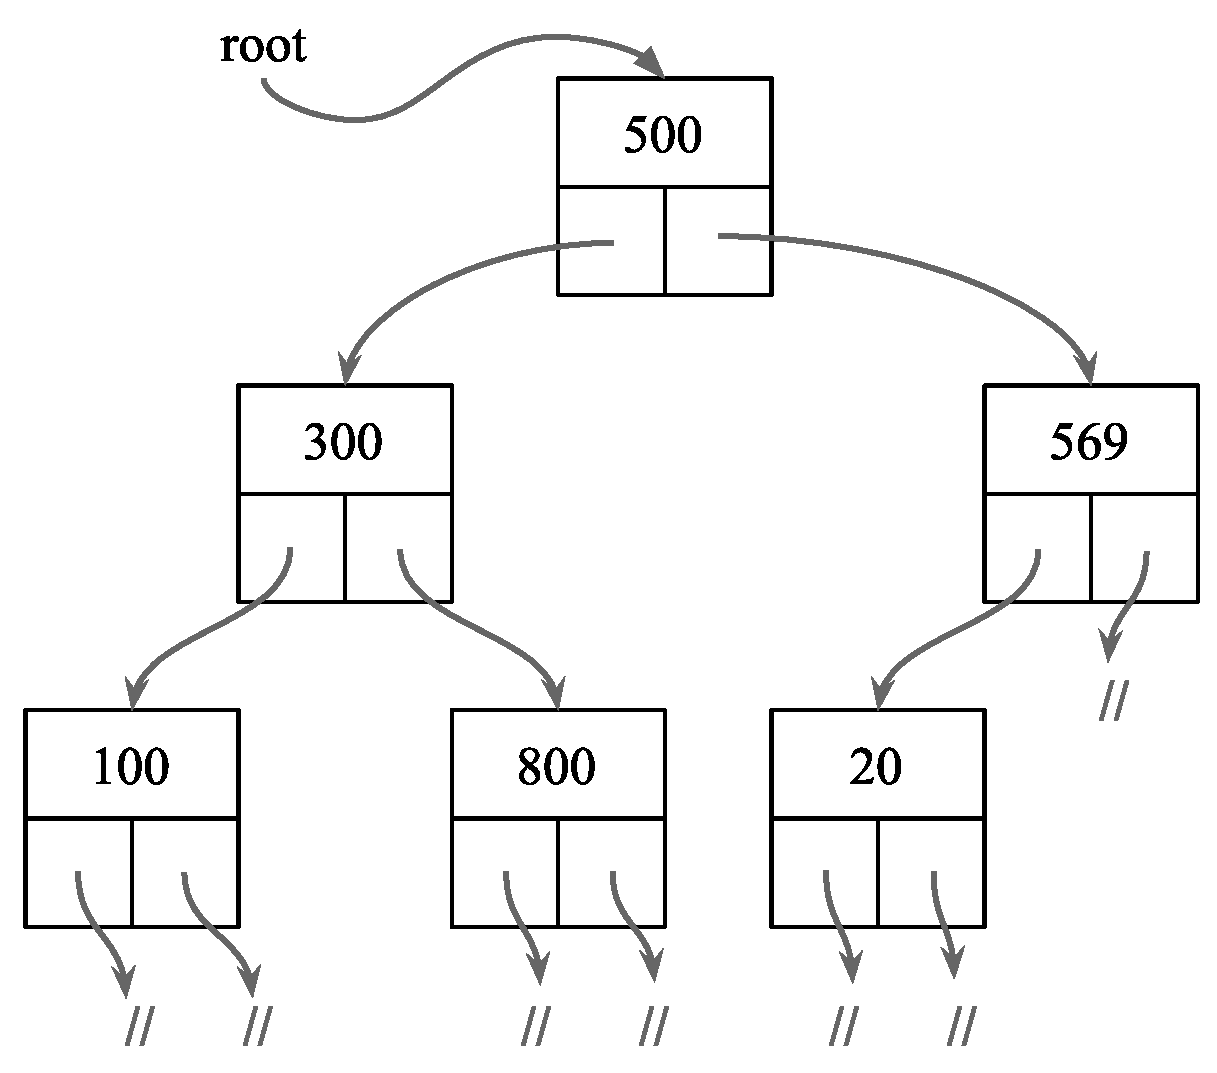
\includegraphics[width=0.5\textwidth]{images/BTPointer.eps}
  \end{center}
  \caption{Representación de un árbol empleando apuntadores. Cada nodo contiene un apuntador a su hijo derecho e izquierdo.}
  \label{fig:BTPointer}
\end{figure}

Así es posible definir un árbol binario como una estructura formada por un nodo vacío o por un nodo simple donde los punteros izquierdo y derecho apuntan a un árbol binario. Entonces, solamente con una variable del tipo Node es posible construir el árbol. Su definición es:
\begin{lstlisting}[upquote=true, language=pseudo]
class Node<T>
public:
  T tInfo
  Node<T>* pLeft
  Node<T>* pRight
end
\end{lstlisting}

En los lenguajes de programación que tienen soporte a apuntadores el valor de éstos pueden estar inicializados con NIL al momento de su creación o en caso contrario se le debe asignar dicho valor. Así, es posible construir una clase un poco más "segura" y en el enfoque orientado a objetos (\textit{mutators} y \textit{observers}) como:
\begin{lstlisting}[upquote=true, language=pseudo]
class Node<T>
private:
  T tInfo
  Node<T>* pLeft
  Node<T>* pRight
public:
  Constructor Node()
    pLeft = NIL
    pRight = NIL
  end

  Constructor Node(T value)
    tInfo = value
  end

  Constructor Node(Node<T>* pRight, pLeft, T tInfo)
    this.pLeft = pLeft
    this.pRight = pRight    
    this.tInfo = tInfo
  end
    
  Destructor Node()
    if pLeft != NULL then
      delete pLeft
    end
    if pRight != NULL then
      delete pRight
    end
  end
  
  void setRightChild(Node<T>* pRight)
    this.pRight = pRight
  end
  
  void setLeftChild(Node<T>* pLeft)
    this.pLeft = pLeft
  end
  
  void setInfo(T tInfo)
    this.tInfo = tInfo
  end
  
  Node<T>* getRightChild()
    return pRight
  end
  
  Node<T>* getLeftChild()
    return pLeft
  end
  
  void getInfo(T tInfo)
    return tInfo
  end
  
end
\end{lstlisting}

%%%%%%%%%%%%%%%%%%%%%%%%%%%%%%
\subsection{Algoritmos}

%%%%%%%%%%%%%%%%%%%%%%%%%%%%%%
\subsubsection{Contar el número de nodos}

\begin{lstlisting}[upquote=true, language=pseudo]
function Count (Node<T>* pNode) : Integer
  if pNode == NIL then
    return 0
  else
    return 1 + Count(*pNode.pRight) + Count(*pNode.pLeft)
  end
end
\end{lstlisting}

%%%%%%%%%%%%%%%%%%%%%%%%%%%%%%
\subsubsection{Buscar el elemento mínimo}

\begin{lstlisting}[upquote=true, language=pseudo]
function Min(Integer a, Integer b) : Integer
  if a > b then
    return b
  end
  return a
end

function isLeaf(Node<Integer>* pNode) : Boolean
  return *pNode.pRight == NIL and *pNode.pLeft
end

function Min (Node<Integer>* pNode) : Integer
  if isLeaf(pNode) then
    return *pNode.tInfo
  else
    return Min(*pNode.tInfo, Min(Min(*pNode.pRight), Min(*pNode.pLeft)))
  end
end
\end{lstlisting}

%%%%%%%%%%%%%%%%%%%%%%%%%%%%%%
\subsubsection{Calcular la profundidad}

\begin{lstlisting}[upquote=true, language=pseudo]
function MaxDepth (Node<T>* pNode) : Integer
  if pNode == NIL then
    return 0
  else
    Integer iLDepth = MaxDepth(*pNode.pLeft)
    Integer iRDepth = MaxDepth(*pNode.pRight)
    if iLDepth > iRDepth then
      return iLDepth + 1
    else
      return iRDepth + 1
  end
end
\end{lstlisting}

%%%%%%%%%%%%%%%%%%%%%%%%%%%%%%
\subsubsection{Árboles binarios iguales}

\begin{lstlisting}[upquote=true, language=pseudo]
function Equals (Node<T>* pNodeA, pNodeB) : Integer
  if pNodeA == NIL and pNodeB == NIL then
    return true
  elseif pNodeA != NIL and pNodeB != NIL then
    return *pNodeA.tInfo == *pNodeB.tInfo and Equals(*pNodeA.pLeft, *pNodeB.pLeft) and Equals(*pNodeA.pRight, *pNodeB.pRight)
  else
    return false
  end
end
\end{lstlisting}


%%%%%%%%%%%%%%%%%%%%%%%%%%%%%%
\subsubsection{Suma de los nodos}

Dado un BST de valores del tipo Integer, se quiere construir una función que sume todos los elementos de los nodos y lo retorne. Una posible función es como sigue:

\begin{lstlisting}[upquote=true, language=pseudo]
function SumAll (Node<Integer>* pNode) : Integer
  if pNode == NIL then
    return 0
  else
    return *pNode.tInfo + SumAll(*pNode.pRight) + SumAll(*pNode.pLeft)
end
\end{lstlisting}

La función verifica en su caso base si es NIL o no. En la parte recursiva, invoca a la función con los nodos derecho e izquierdo. Ahora, si un nodo del árbol no tiene hijos, o solo tiene hijo derecho, o solo tiene hijo izquierdo entonces cuando se genere el ambiente recursivo habrá de retornar 0 por el caso base (debido a que no aporta en la suma). Este enfoque puede resultar ineficiente debido a que si una de las ramas del nodo es NIL, entonces no es necesario invocar a la función. Por ejemplo, para un árbol completo de altura $h$ se realizarán $2^{h+1}$ invocaciones que siempre retornarán 0 (i.e. los nodos hojas).

Entonces, sería ideal primero verificar el número de hijos que posee un nodo para no hacer invocaciones que no aporten al cómputo (la suma final). A continuación se muestra una nueva versión donde se toma en cuenta dichos aspectos, siendo más eficientes en solo generar las invocaciones necesarias para el cálculo.

\begin{lstlisting}[upquote=true, language=pseudo]
function isLeaf(Node<Integer>* pNode) : Boolean
  return *pNode.pRight == NIL and *pNode.pLeft
end

function SumAll (Node<Integer>* pNode) : Integer
  if pNode != NIL then
    if isLeaf(pNode) then
      return *pNode.tInfo
    elseif *pNode.pRight == NIL then
      return *pNode.tInfo + SumAll(*pNode.pLeft)
    elseif *pNode.pLeft == NIL then
      return *pNode.tInfo + SumAll(*pNode.pRight)
    else
      return *pNode.tInfo + SumAll(*pNode.pRight) + SumAll(*pNode.pLeft)
  end
  return 0	//solo se debería invocar si el árbol es vacío
end
\end{lstlisting}

%%%%%%%%%%%%%%%%%%%%%%%%%%%%%%%%%%%%%%%%%%%%%%%%%%%%%%%
\section{Binary Search Tree - BST}

Un tipo Binary Search Tree (BST), árbol binario de búsqueda, es un árbol binario con la característica de que todos los elementos almacenados en el subárbol izquierdo de cualquier nodo $k$ son menores al valor del elemento almacenado en $k$, y que todos los elementos almacenados en el subárbol derecho de $k$ son mayores que el valor del elemento almacenado en $k$. La Fig. \ref{fig:BSTExample1} muestra un ejemplo de dos BST empleando un mismo conjunto de números.

\begin{figure}[htpb!]
  \begin{center}
    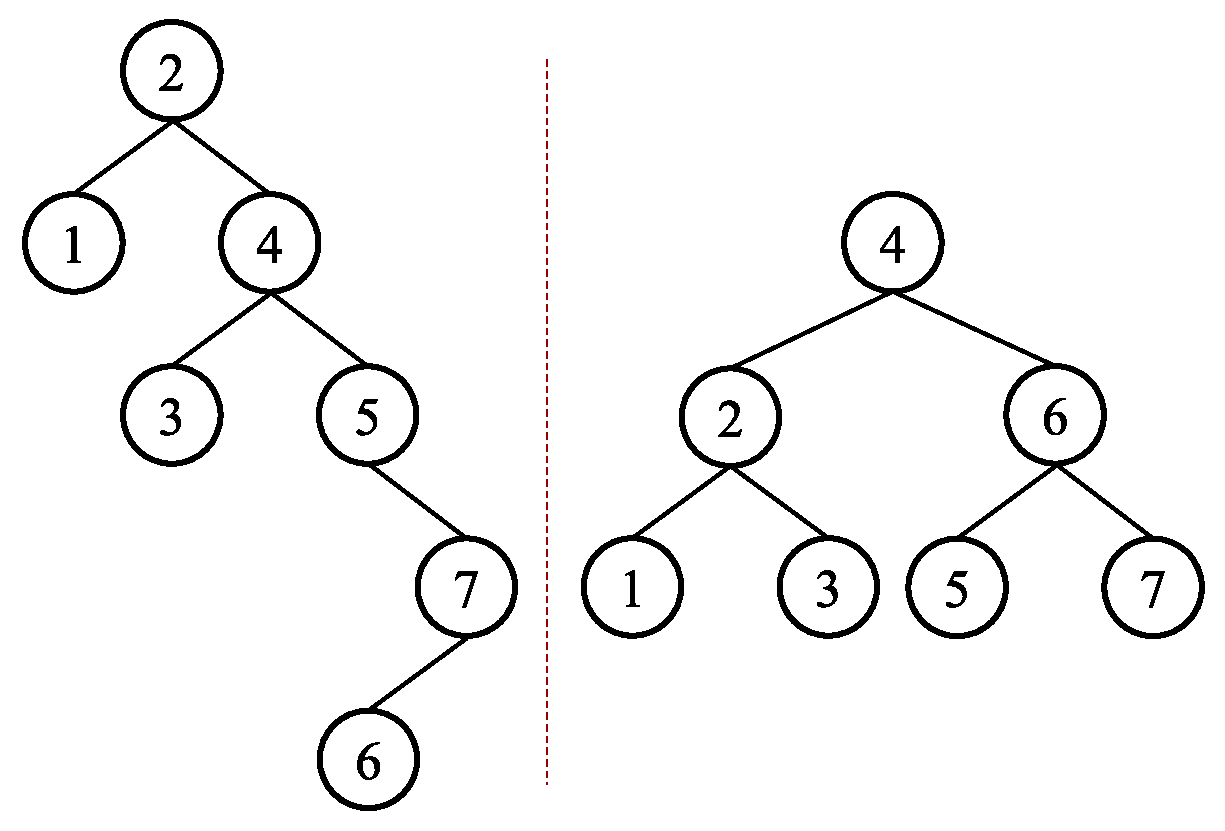
\includegraphics[width=0.6\textwidth]{images/BSTExample1.eps}
  \end{center}
  \caption{Ejemplo de dos BST para un mismo conjunto de números.}
  \label{fig:BSTExample1}
\end{figure}

En un BST, para todo nodo existe una clave única que lo identifica, es decir, no hay repeticiones en el valor discriminante para la comparación. Un nodo puede almacenar diversos valores propios de la estructura de datos, pero requiere solo un valor que sirva de clave (key) y pueda ser aplicador el operador de comparación (mayor que, menor que). De esta forma existe una relación de orden total en el tipo asociado al key. Así por definición, para cada nodo las claves de los nodos de su subárbol izquierdo siempre son menores y las del subárbol derecho siempre son mayores.

El recorrido en inorder de un BST produce la secuencia de claves en orden ascendente. Por ejemplo, para los dos árboles de la Fig. \ref{fig:BSTExample1} se produce la secuencia $1, 2, 3, 4, 5, 6, 7$. Por su lado, el recorrido inorder en reverso produce la secuencia en orden descendente.

La diferencia observada en los árboles del ejemplo se debe a que su forma viene dada por el orden en que aparecen las claves de la secuencia (del 1 al 7) al momento de construir el BST. A pesar de que los árboles tengan las mismas claves y el mismo orden en recorrido inorder, ambos tuvieron una secuencia de inserción distinta. Para el primer árbol (izquierda) el primer valor de la secuencia fue el 2, para el segundo (derecha) el primer valor fue el 4.


%%%%%%%%%%%%%%%%%%%%%%%%%%%%%%
\subsection{Especificación}

Las operaciones de Insert (inserción) y Lookup (búsqueda) en un árbol binario de búsqueda suelen ser rápidas. En promedio, un algoritmo de búsqueda en un árbol binario puede localizar un nodo en un árbol de $n$ nodos en un orden de complejidad de $log(N)$ (logaritmo base 2). Por lo tanto, un BST son estructuras ideales para problemas de "diccionario" donde un código/id es insertado y se busca su información asociada de forma eficiente. El comportamiento logarítmico es para el caso promedio, es posible que para un árbol en particular sea más lento (dependiendo de su forma).

A continuación se muestra una posible especificación para la definición de la clase BST.

\begin{lstlisting}[upquote=true, language=pseudo]
class Node<T>
public:
  T tInfo
  Node<T>* pLeft
  Node<T>* pRight
end

class BST<T>
private:
  Node<T>* pRoot
public:
  Constructor BST()
  Destructor BST()
  function GetRoot() : Node<T> *
  function IsEmpty() : Boolean
  function Lookup(Node<T>* pNode, T tInfo) : Boolean  		//puede retornar un Node<T>*
  function Insert (Node<T>* pNode, T tInfo) : Node<T> * 	//puede retornar un Boolean
  void Delete(Node<T>* pNode, T tInfo)
end
\end{lstlisting}

Es posible que la operación de Lookup retorne un tipo $Node<T>*$ en vez de un tipo Boolean (igual con la función Insert). De esa forma permitirá localizar un elemento dentro del BST, o retornar NIL que indica que el elemento no existe.

%%%%%%%%%%%%%%%%%%%%%%%%%%%%%%
\subsection{Implementación}

A continuación se muestra la implementación de la clase BST. Se mostrará las funciones con una breve explicación de cada una.

La implementación inicial de la clase BST consiste en el constructor, destructor, la función que retorna la raíz y verificar si el árbol es vacío o no. Todas estas funciones son muy similares en todas las estructuras dinámicas.

\begin{lstlisting}[upquote=true, language=pseudo]
class BST<T>
public:
  
  Constructor BST()
    pRoot = NIL
  end
  
  Destructor BST()
  end
  
  function GetRoot() : Node<T> *
    return pRoot
  end
  
  function IsEmpty() : Boolean 
    return pRoot == NIL
  end
\end{lstlisting}

Dado un BST y un valor se quiere verificar si dicho valor existe o no en el árbol. El patrón básico de la función Lookup ocurre de forma recursiva (como es usual en los algoritmos de árboles): 
\begin{enumerate}
\item Tratar con el caso base donde el árbol es vacío
\item Tratar con el nodo actual y emplear la recursión para tratar con sus subárboles
\end{enumerate}

Dado que el árbol es un BST, se tiene un orden que se evalua mediante operaciones relacionales y decide si trata del árbol derecho o el árbol izquierdo.

\begin{lstlisting}[upquote=true, language=pseudo]
  function Lookup (Node<T>* pNode, T tInfo) : Boolean
    if pNode == NIL then
      return false
    else
      select
        tInfo < *pNode.tInfo: return Lookup (*pNode.pLeft, tInfo)
        tInfo > *pNode.tInfo: return Lookup (*pNode.pRight, tInfo)
        tInfo == *pNode.tInfo: return true
      end
    end
  end
\end{lstlisting}

El proceso de inserción consiste en dado el BST y una clave/información colocarla en el lugar correcto. Se retorna el apuntador de la posición donde fue insertado. Para ello se realizan los siguientes pasos:
\begin{itemize}
\item Si el BST es vacío, se crea el nodo raíz del árbol
\item Si el BST tenía al menos la raíz, se verifica dónde se debe insertar el nodo nuevo recorriendo el árbol desde la raíz, y descendiendo por la rama izquierda si el valor a insertar es menor o por la derecha si es mayor que el nodo raíz actual en cada invocación recursiva.
\item Si la clave/información a insertar ya se encuentra en el árbol se debe verificar de alguna forma (i.e. mensaje de error, retorna NIL, etc). En la implementación mostrada se asume que no habrá claves repetidas pero \textbf{no inserta} un nodo nuevo.
\item Si la clave/información no existe en el árbol, se crea un nodo nuevo como el paso 1 y se inserta siempre como una hoja hija derecha o izquierda del nodo hallado en el paso 2.
\end{itemize}

La Fig. \ref{fig:BSTInsert} muestra de forma gráfica el proceso de insertar los elementos 11, 6, 8, 19, 4, 10, 5, 17 (en ese orden) en un BST.

\begin{figure}[htpb!]
  \begin{center}
    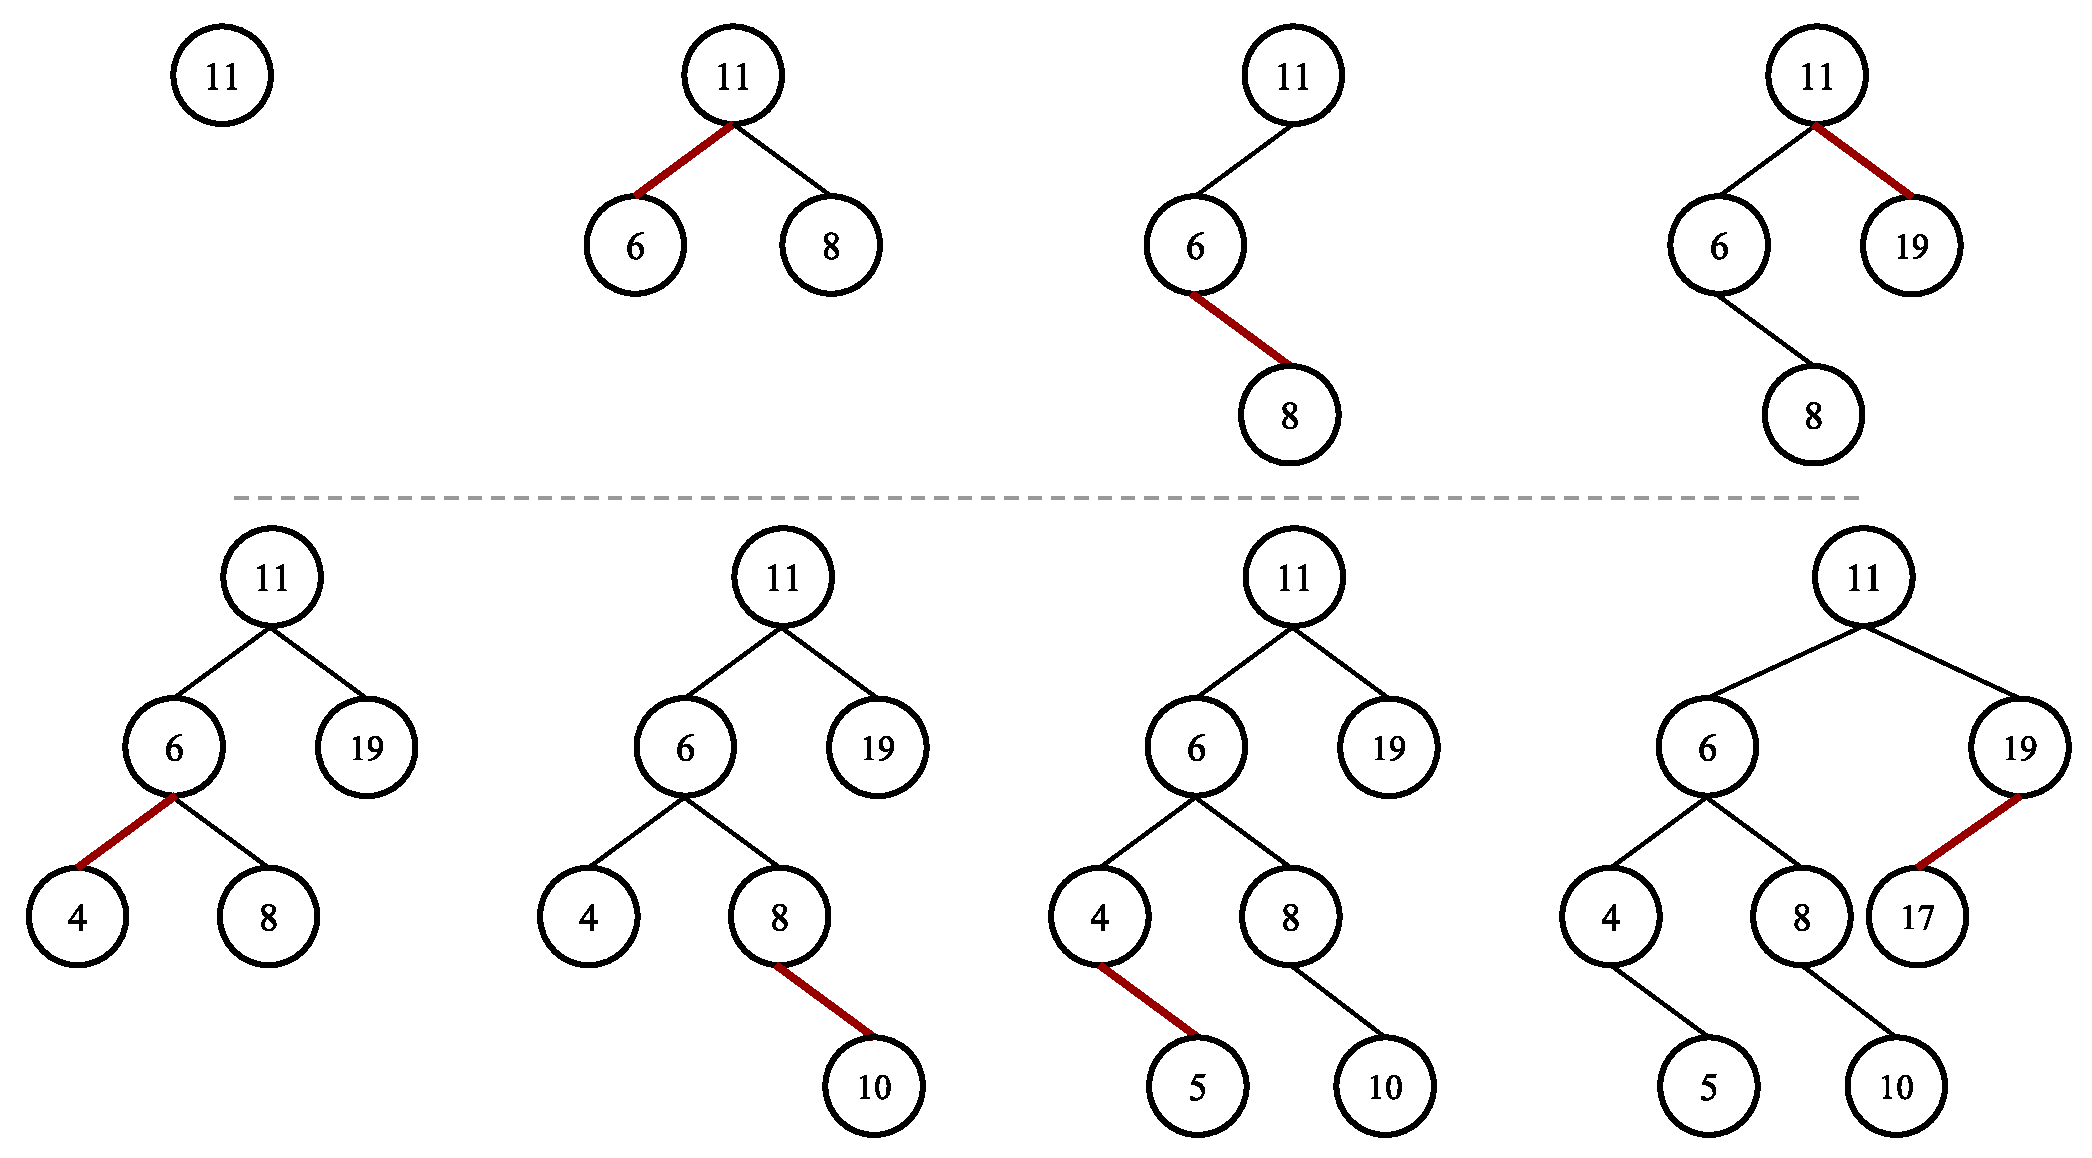
\includegraphics[width=1.0\textwidth]{images/BSTInsert.eps}
  \end{center}
  \caption{Proceso de inserción de los elementos 11, 6, 8, 19, 4, 10, 5, 17 en un BST.}
  \label{fig:BSTInsert}
\end{figure}

Es importante destacar que la forma del árbol depende del orden en el cual los nodos son insertados.

\begin{lstlisting}[upquote=true, language=pseudo]
  function Insert (Node<T>* pNode, T tInfo) : Node<T> *
    if pNode == NIL then
      Node<T>* pNew = new Node
      *pNew.tInfo = tInfo
      *pNew.pLeft = *pNew.pRight = NIL
      return pNew
    else
      select
        tInfo < *pNode.tInfo:
          *pNode.pLeft = Insert(pNode->pLeft, tInfo)
        tInfo > *pNode.tInfo:  
          *pNode.pRight = Insert(pNode->pRight, tInfo)
        tInfo == *pNode.tInfo:
          return pNode	//se asume que no hay claves repetidas en el BST
      end
      return pNode
    end
  end
\end{lstlisting}

Para la operación Delete en un BST se deben considerar 3 casos posibles en cuanto a la ubicación de un nodo:
\begin{itemize}
\item El nodo a eliminar es hoja (no tiene hijos): En este caso se elimina el nodo sin
mayores problemas.
\item El nodo a eliminar tiene solo un hijo o subárbol (izquierdo o derecho): Se reenlaza
al padre del nodo a eliminar con el hijo existente.
\item El nodo a eliminar tiene dos hijos: En este caso se debe buscar:
a) El nodo de mayor clave en su subárbol izquierdo (gráficamente el nodo más a la
derecha del subárbol).
b) El nodo de menor clave en su subárbol derecho (gráficamente el nodo más a la
izquierda del subárbol).
La clave de este nodo se le asigna al nodo pasado a la función y posteriormente
se elimina el nodo.
\end{itemize}

Fig. \ref{fig:delsbt1}

%\begin{figure}[htpb!]
%  \begin{center}
%    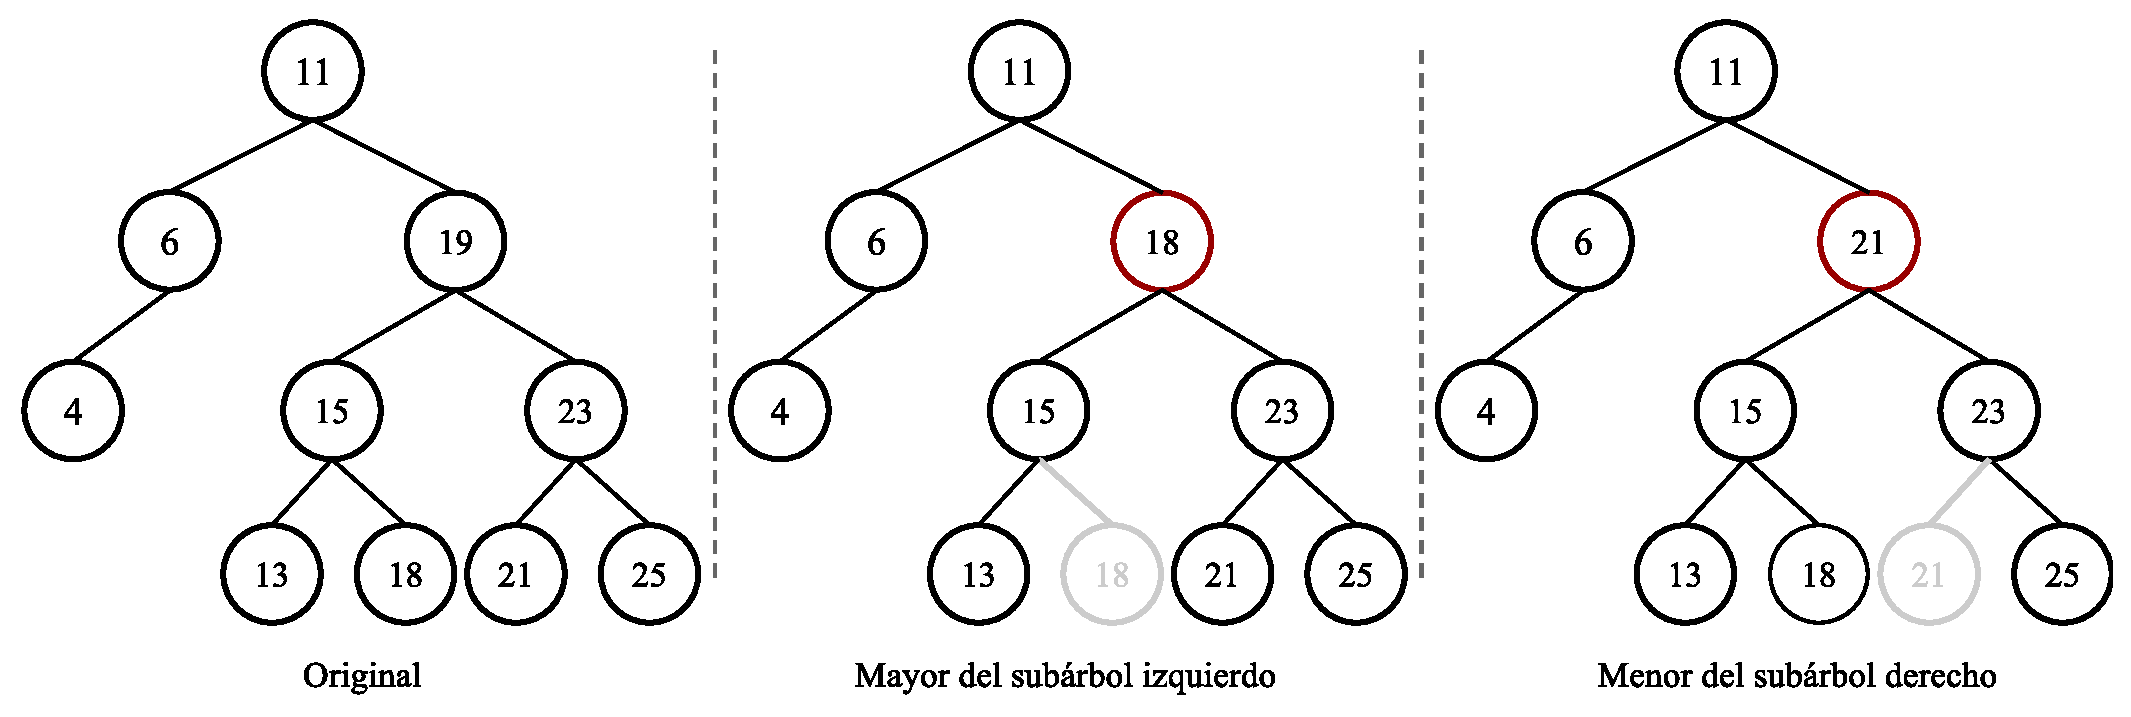
\includegraphics[width=1.0\columnwidth]{images/BSTDelete1.eps}
%  \end{center}
%  \caption{Representación de la eliminación del mayor de los nodos menores o, el menor de los nodos mayores en un BST.}
%  \label{fig:delsbt1}
%\end{figure}

\begin{lstlisting}[upquote=true, language=pseudo]  
  void DelMax(ref Node<T>* pNode, ref T tInfo)
    if *pNode.pRight != NIL then
      DelMax(ref *pNode.pRight, ref tInfo)
    else
      Node<T>* pTemp = pNode
      tInfo = *pNode.tInfo
      pNode = *pNode.pLeft
    end
  end
  
  void Delete(Node<T>* pNode, T tInfo)
    if pNode != NIL then
      select
        tInfo < *pNode.tInfo:
          Delete(*pNode.pLeft, tInfo)
        tInfo > *pNode.tInfo:
          Delete(*pNode.pRight, tInfo)
        tInfo == *pNode.tInfo:
          Node<T>* pTemp = pNode
          select
            *pNode.pLeft == NIL and *pNode.pRight == NIL:	//no tiene hijos
              pNode = NIL
              delete pTemp
            *pNode.pLeft == NIL and *pNode.pRight != NIL:	//tiene hijo derecho
              pNode = *pNode.pRight
              delete pTemp
            *pNode.pLeft != NIL and *pNode.pRight == NIL:	//tiene hijo izquierdo
              pNode = *pNode.pLeft
              delete pTemp
            *pNode.pLeft != NIL and *pNode.pRight != NIL:	//tiene ambos hijos
              DelMax(ref pNode, ref *pNode.tInfo)
              //*pNode.tInfo = tInfo
              //pTemp = FindMin(pNode)
              //*pNode.tInfo = *pTemp.tInfo
              //Delete(pTemp, tInfo)
          end
      end
    end
  end
end
\end{lstlisting}

Given a non-empty binary search tree, 
 return the minimum data value found in that tree. 
 Note that the entire tree does not need to be searched.

\begin{lstlisting}[upquote=true, language=pseudo]
function MinValue (Node<T>* pNode) : Integer
  Node<T>* pTemp = pNode
  while (*pTemp.pLeft != NIL) do
    pTemp = *pTemp.pLeft
  end
  return *pTemp.tInfo
end
\end{lstlisting}

Returns true if a binary tree is a binary search tree. 
\begin{lstlisting}[upquote=true, language=pseudo]
function IsBST (Node<T>* pNode) : Boolean
  if pNode == NIL then
    return true
  end
  
end
\end{lstlisting}

\subsection{Problema de Desequilibrio}

El orden de inserción en un BST determina la forma estructural del árbol. La Fig. \ref{fig:BSTDesequilibrado} muestra un ejemplo de distintos tipos de inserción en un BST del tipo Char, siendo insertados de izquierda a derecha.

\begin{figure}[htpb!]
  \begin{center}
    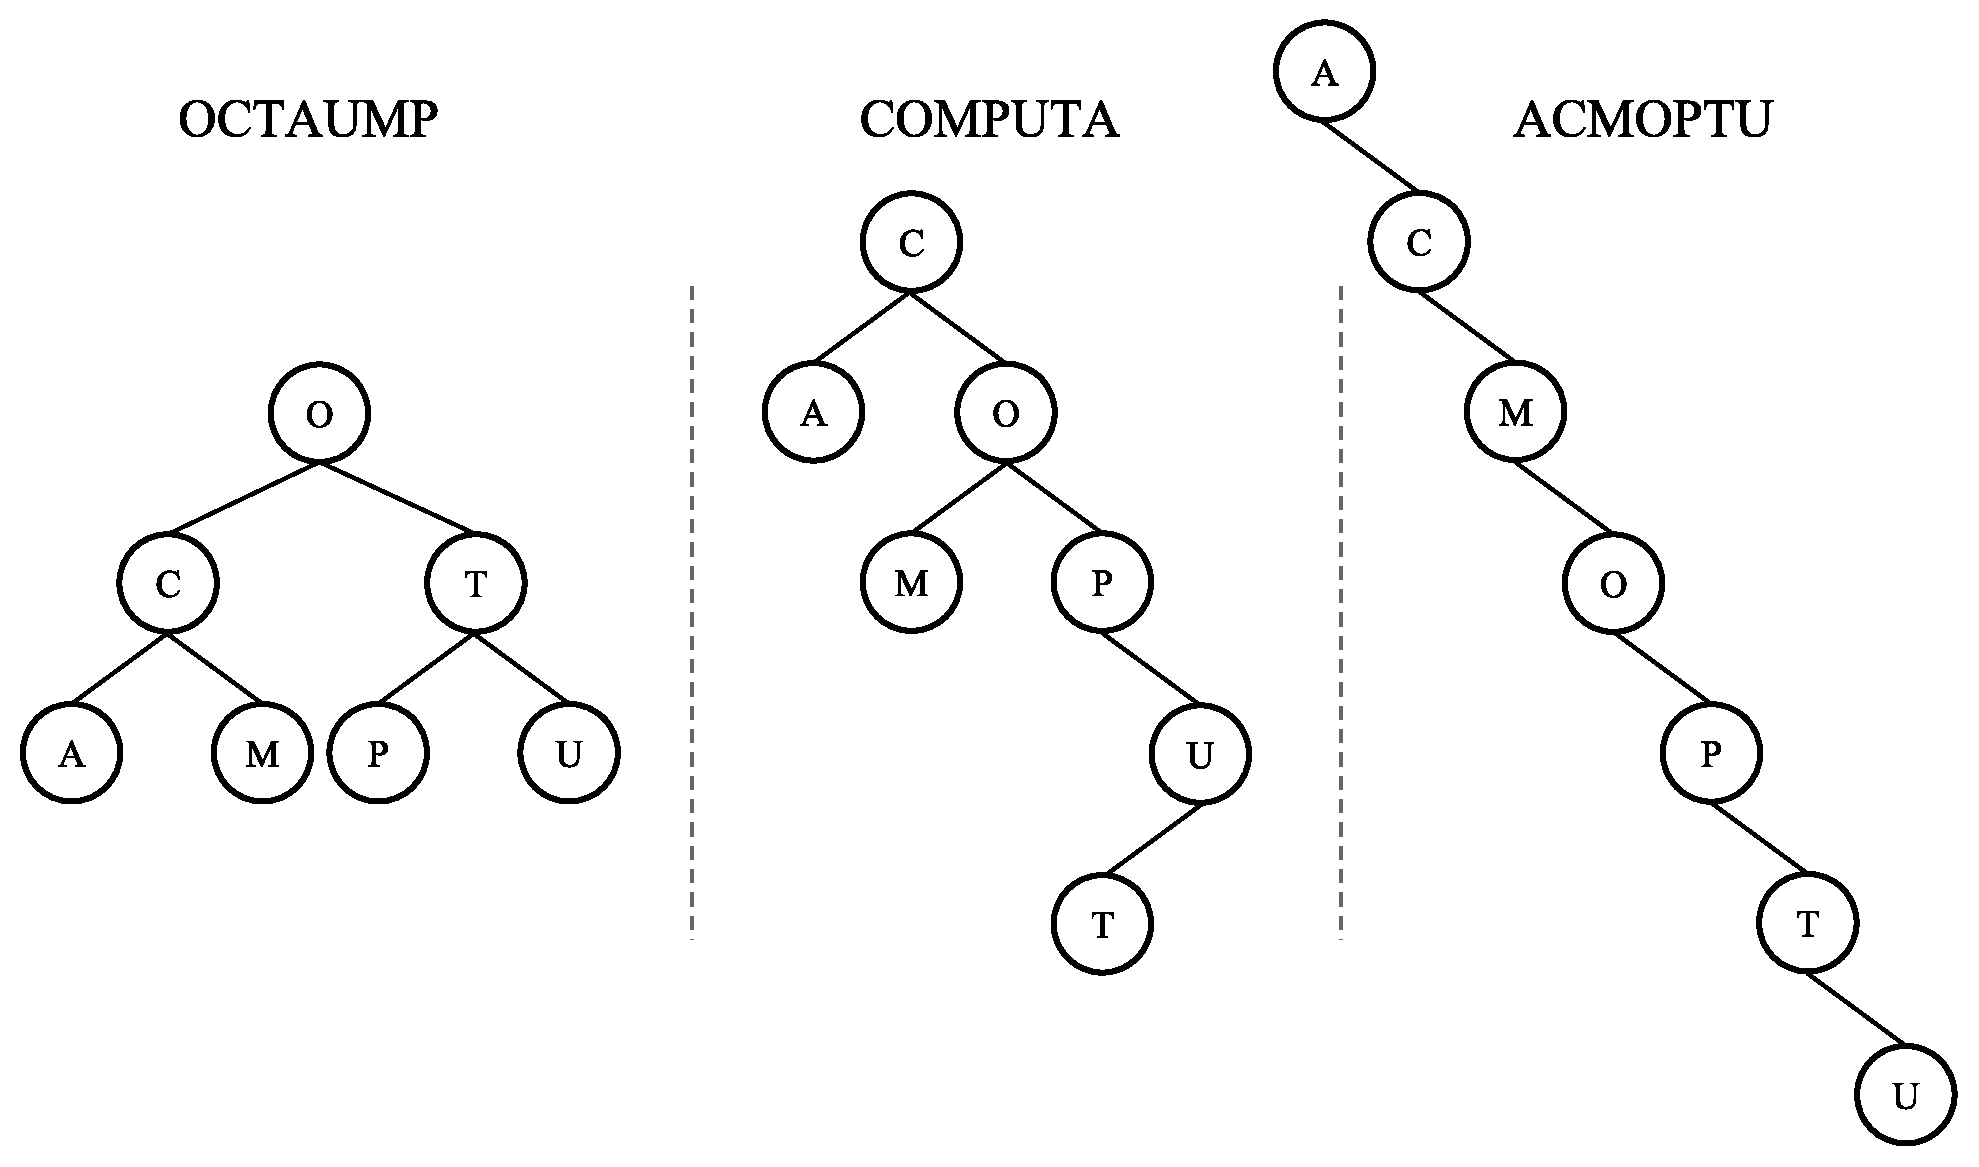
\includegraphics[width=0.9\textwidth]{images/BSTDesequilibrado.eps}
  \end{center}
  \caption{Ejemplo de 3 tipos de BST generados con el mismo conjunto de datos en diferente orden.}
  \label{fig:BSTDesequilibrado}
\end{figure}

Dado este aspecto, si los nodos de un BST son insertados en orden creciente (3er caso de la Fig. {fig:BSTDesequilibrado}) el árbol crecerá solo hacia el lado derecho como una lista simplemente enlazada, y todos los apuntadores izquierdos serán NIL. Del mismo modo, si son insertados en orden decreciente ('U','T','P','O','M','C','A'). La forma de una lista enlazada "degrada" la complejidad logarítimica del árbol.

Por el motivo anterior, es ideal construir un mecanismo que no permita construir árboles de búsqueda que sean degradados sino conseguir árboles tan balanceados como sea posible. Por ello estudiaremos AVL y XXX.

%%%%%%%%%%%%%%%%%%%%%%%%%%%%%%%%%%%%%%%%%%%%%%%%%%%%%%%%
\section{AVL}

Un árbol AVL, llamado así por el nombre de sus inventores Georgy \textbf{A}delson-\textbf{V}elsky y Evgenii \textbf{L}andis, es un BST que se "auto" balancea, es decir, cuando se inserta o remueve un nodo se aplican operaciones que tratan de mantener el árbol balanceado. En un árbol AVL, las alturas de los subárboles de cualquier nodo difiere a lo sumo en 1, y en caso de no cumplirse esto se debe re-balancear para mantener dicha propiedad. Entonces, en la condición de los árboles AVL se considera un factor de equilibrio (\textit{balance}):
$balanceFactor = height(left) - height(right)$

En la Fig. \ref{fig:AVLExample1} se muestra un ejemplo de 3 árboles AVL. El valor dentro de cada nodo (en esta ilustración) representa el factor de equilibrio de cada nodo, donde los valores positivos indican que la altura del subárbol izquierdo es mayor a la altura del subárbol derecho, y nos negativos el caso contrario. El factor de equilibrio 0 significa que ambos subárboles tienen la misma altura.

\begin{figure}[htpb!]
  \begin{center}
    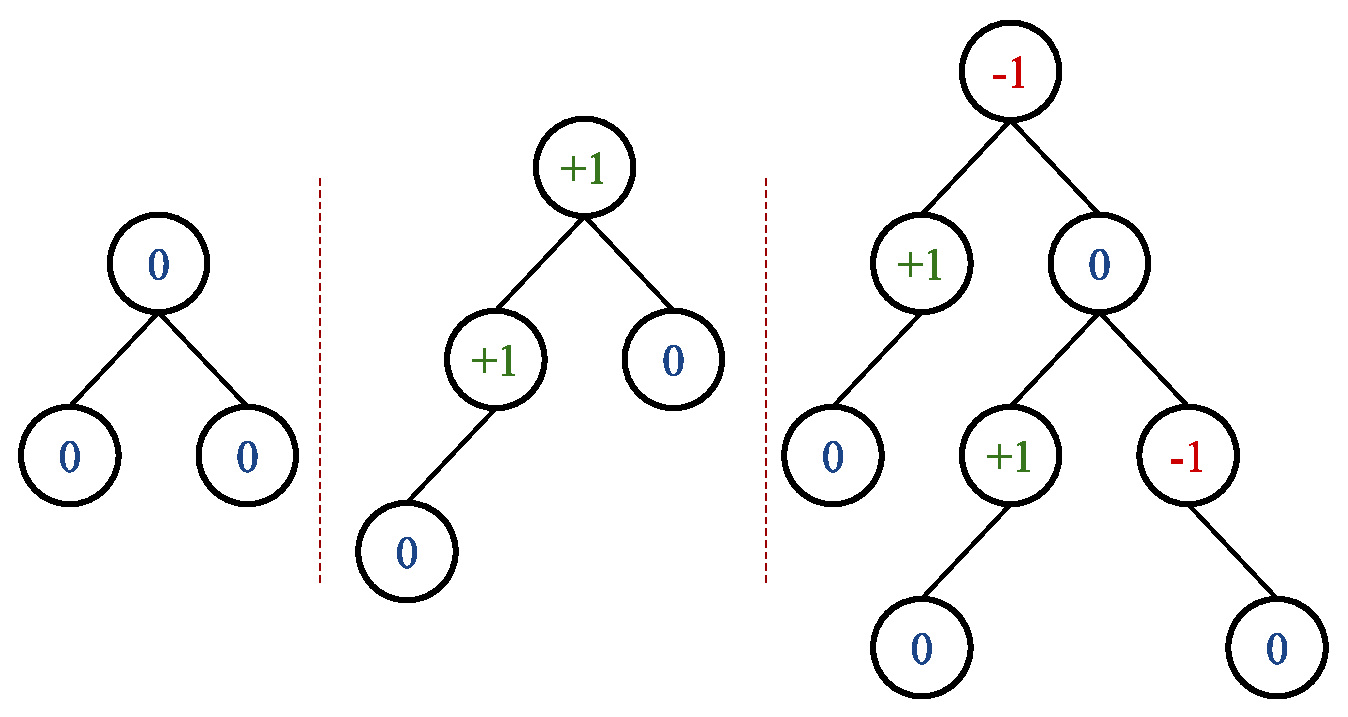
\includegraphics[width=0.8\textwidth]{images/AVLExample1.eps}
  \end{center}
  \caption{Ejemplo de tres árboles AVL mostrando su factor de equilibrio.}
  \label{fig:AVLExample1}
\end{figure}

\begin{figure}[htpb!]
  \begin{center}
    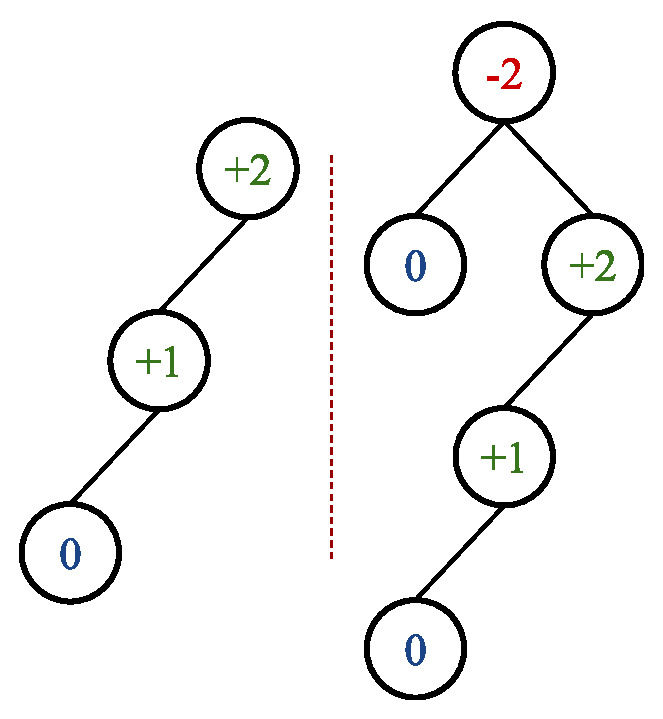
\includegraphics[width=0.4\textwidth]{images/AVLExample2.eps}
  \end{center}
  \caption{Representación en forma de árbol del ejemplo de código en HTML.}
  \label{fig:AVLExample2}
\end{figure}

\subsection{Rotaciones}

\begin{figure}[htpb!]
  \begin{center}
    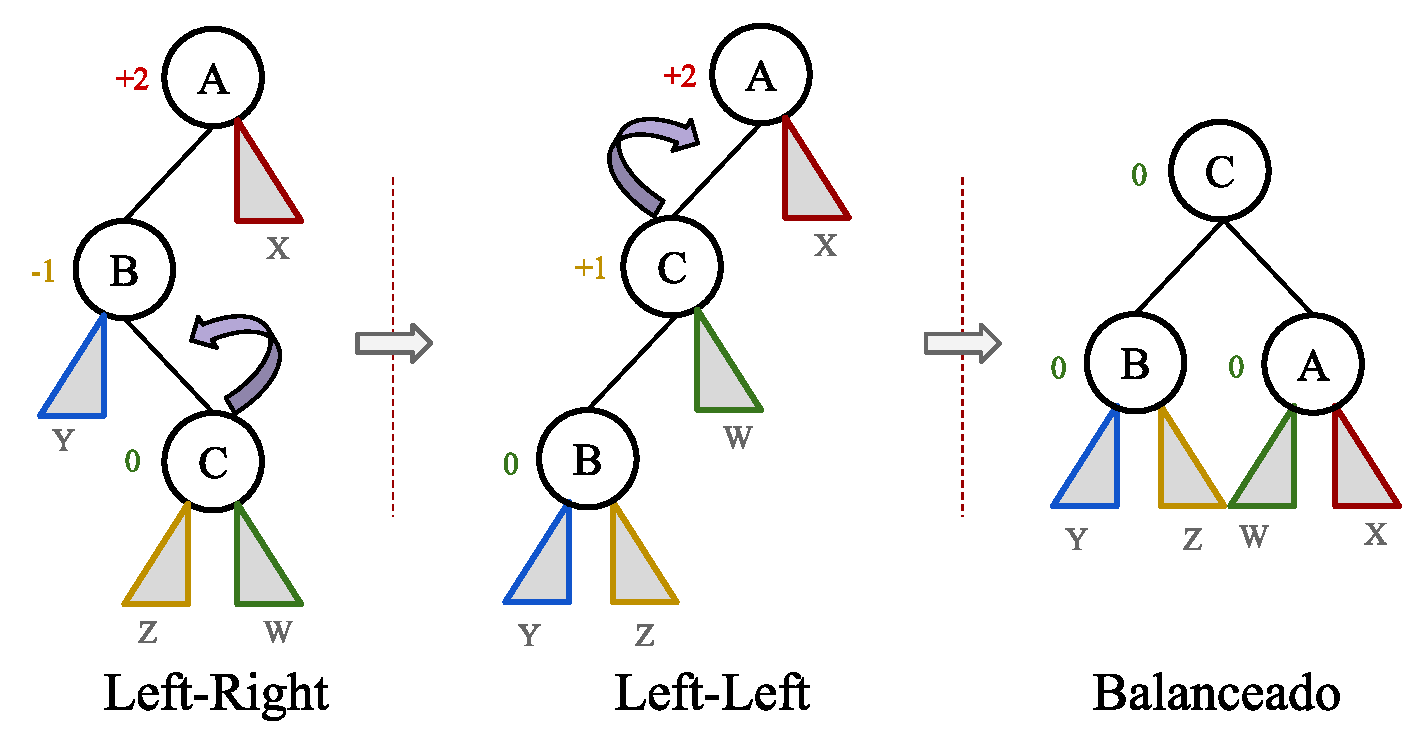
\includegraphics[width=1.0\textwidth]{images/AVLRotation1.eps}
  \end{center}
  \caption{Representación en forma de árbol del ejemplo de código en HTML.}
  \label{fig:AVLRotation1}
\end{figure}

\begin{figure}[htpb!]
  \begin{center}
    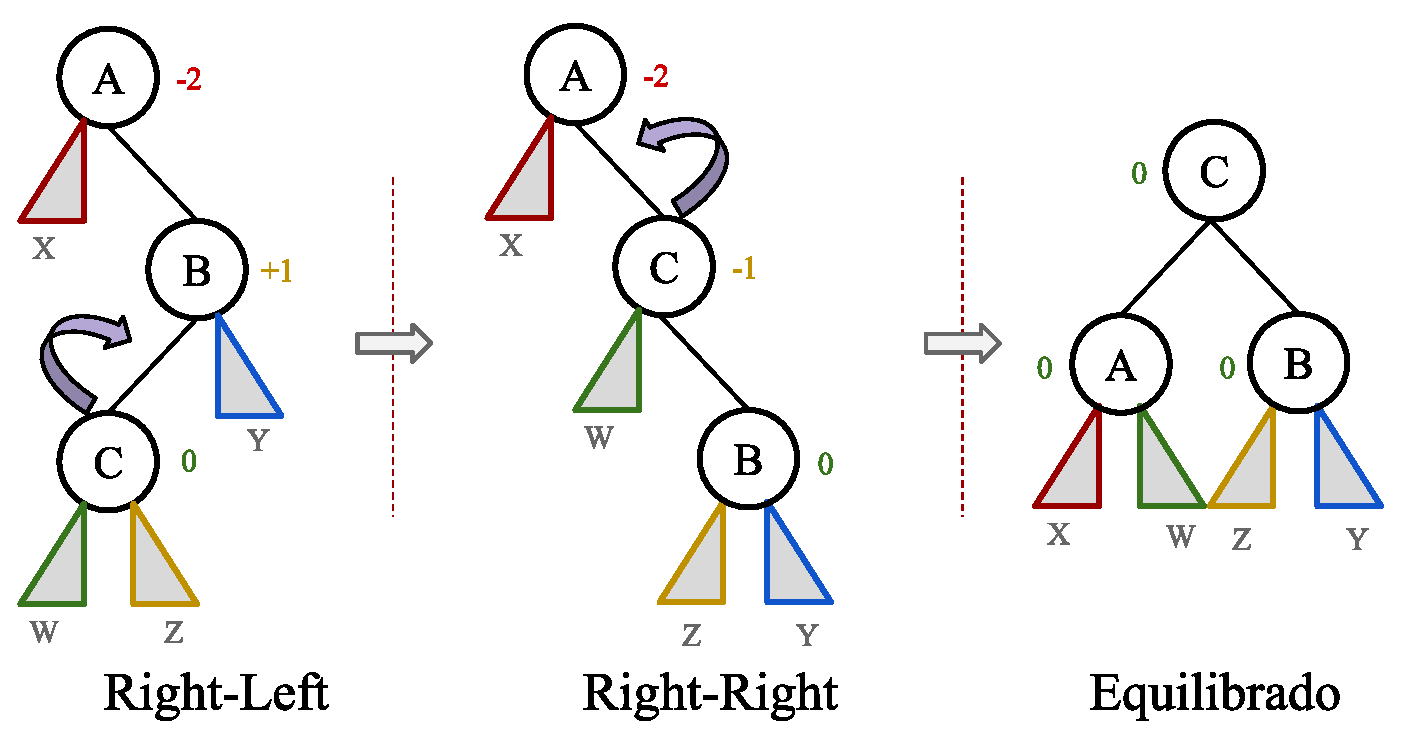
\includegraphics[width=1.0\textwidth]{images/AVLRotation2.eps}
  \end{center}
  \caption{Representación en forma de árbol del ejemplo de código en HTML.}
  \label{fig:AVLRotation2}
\end{figure}

\subsection{Insertar}

\begin{figure}[htpb!]
  \begin{center}
    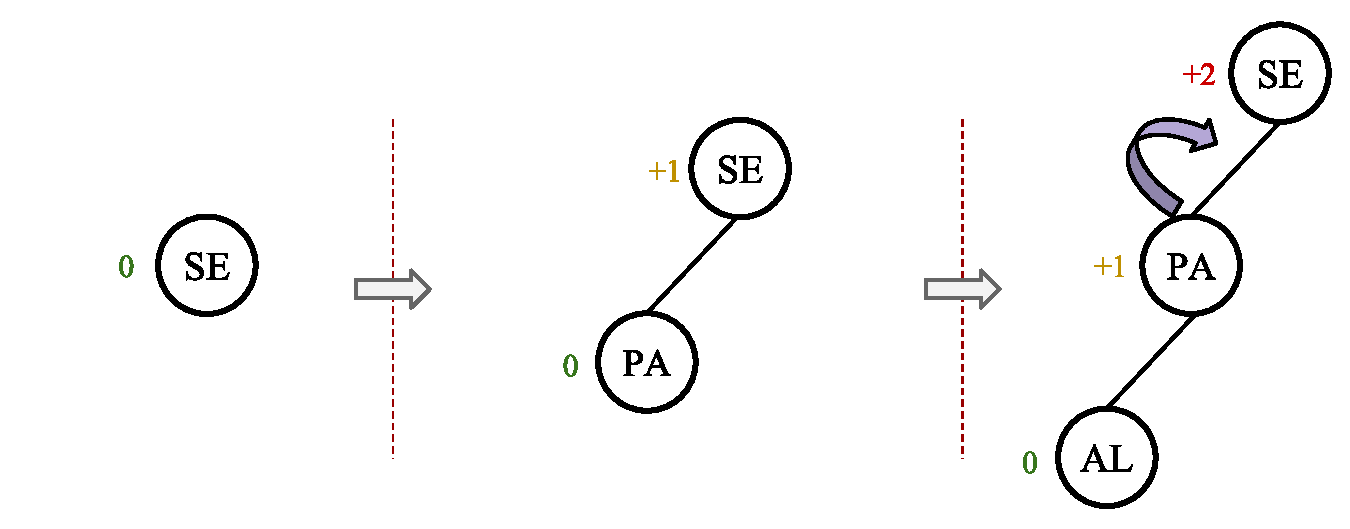
\includegraphics[width=1.0\textwidth]{images/AVLInsertion1.eps}
  \end{center}
  \caption{Representación en forma de árbol del ejemplo de código en HTML.}
  \label{fig:AVLInsertion1}
\end{figure}

\begin{figure}[htpb!]
  \begin{center}
    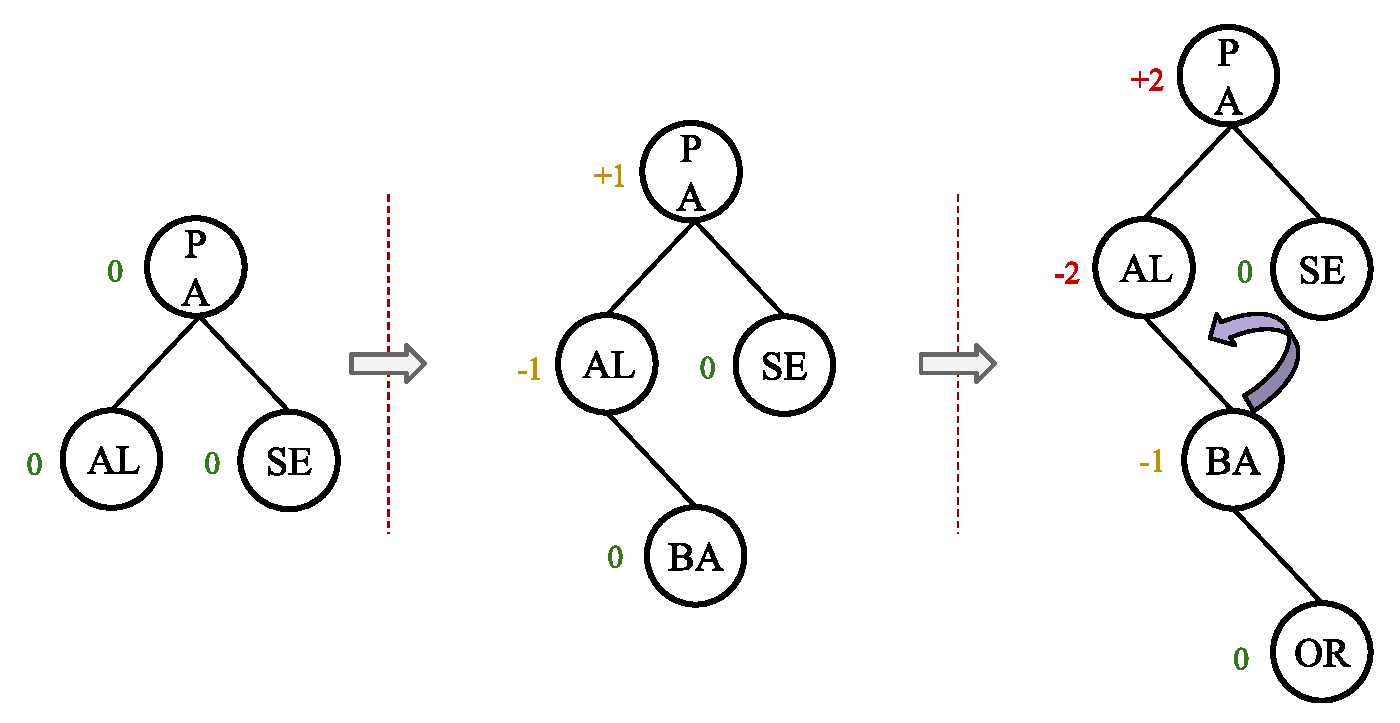
\includegraphics[width=1.0\textwidth]{images/AVLInsertion2.eps}
  \end{center}
  \caption{Representación en forma de árbol del ejemplo de código en HTML.}
  \label{fig:AVLInsertion2}
\end{figure}

\begin{figure}[htpb!]
  \begin{center}
    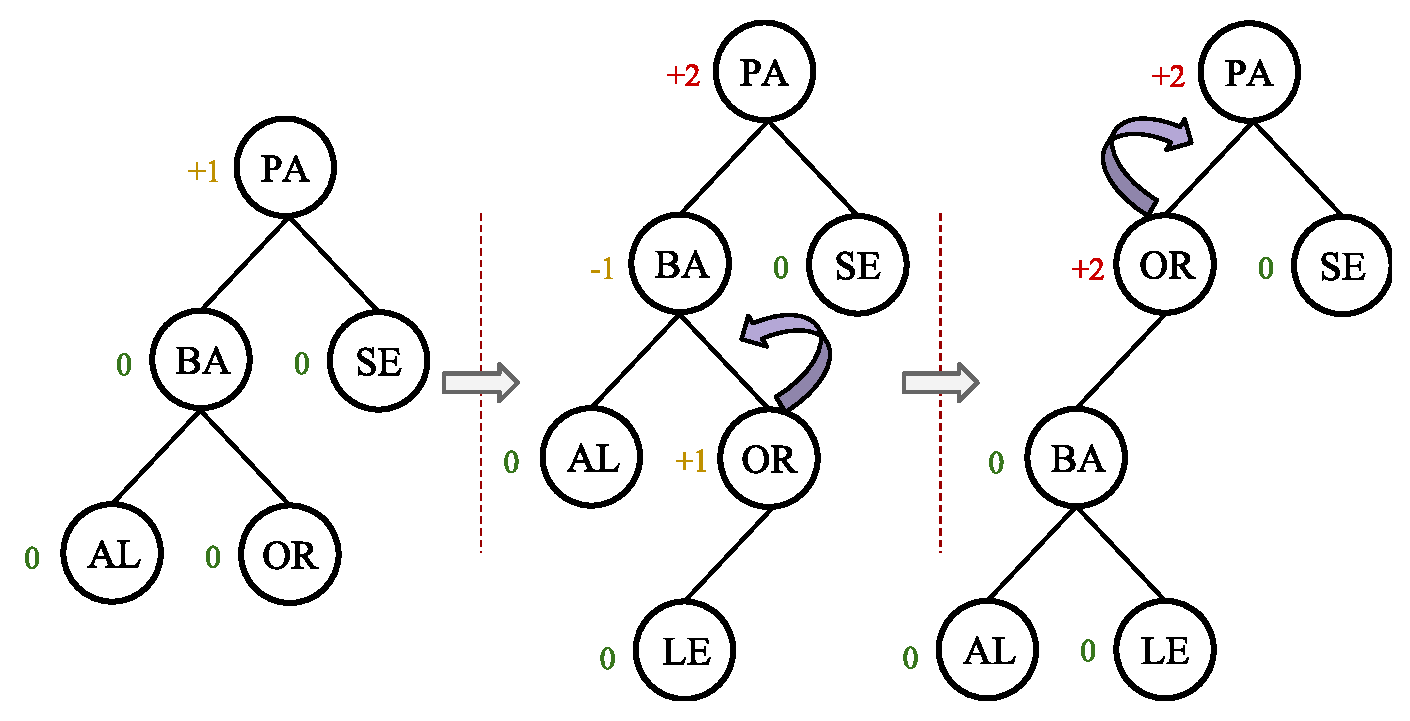
\includegraphics[width=1.0\textwidth]{images/AVLInsertion3.eps}
  \end{center}
  \caption{Representación en forma de árbol del ejemplo de código en HTML.}
  \label{fig:AVLInsertion3}
\end{figure}

\begin{figure}[htpb!]
  \begin{center}
    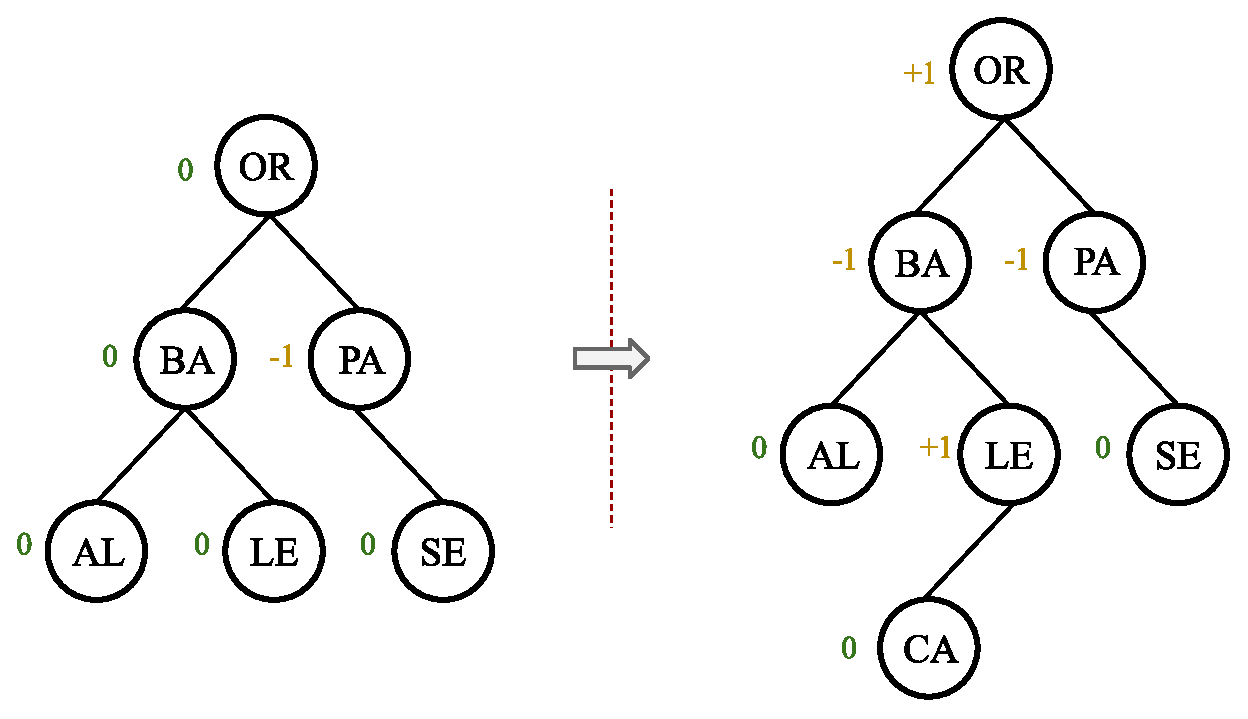
\includegraphics[width=0.8\textwidth]{images/AVLInsertion4.eps}
  \end{center}
  \caption{Representación en forma de árbol del ejemplo de código en HTML.}
  \label{fig:AVLInsertion4}
\end{figure}


\begin{figure}[htpb!]
  \begin{center}
    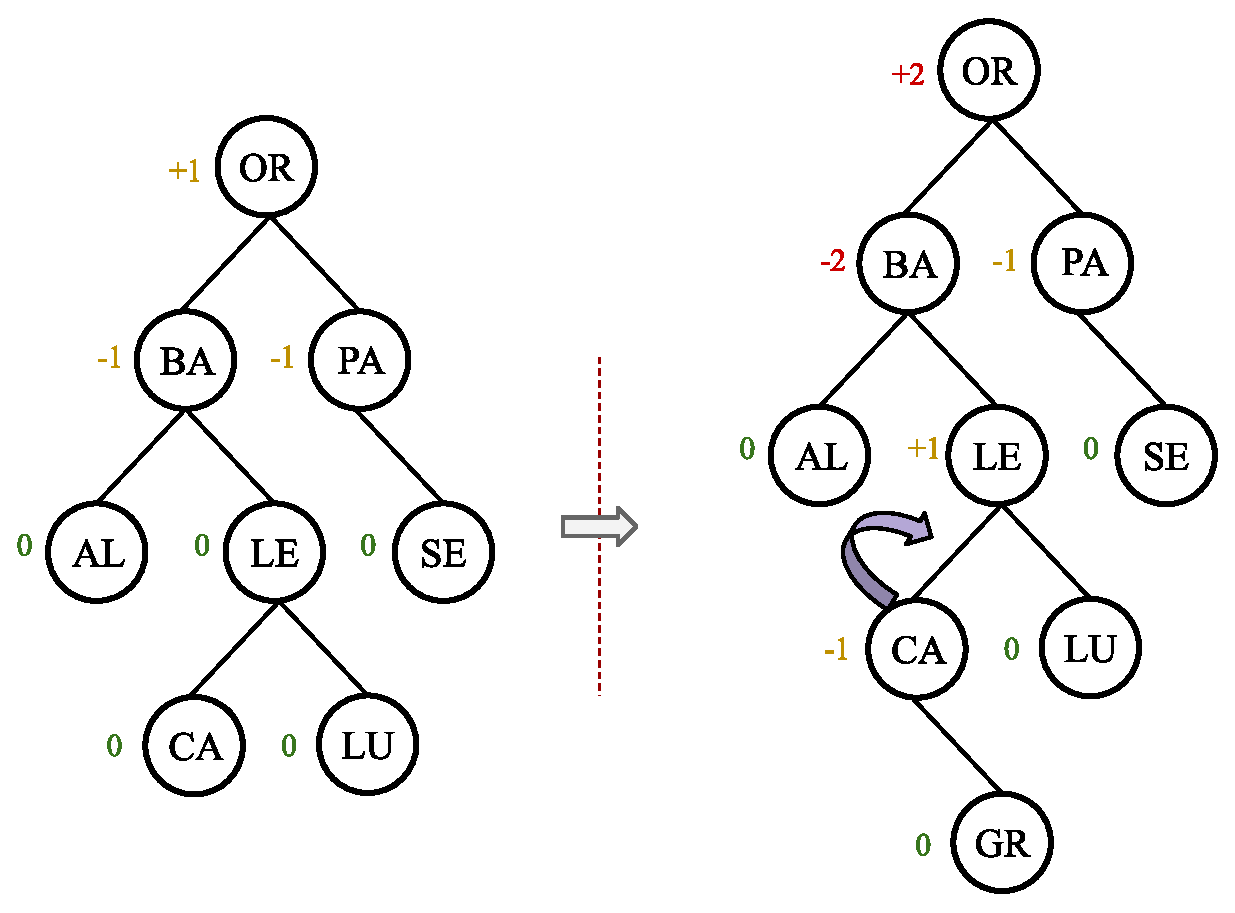
\includegraphics[width=0.7\textwidth]{images/AVLInsertion5.eps}
  \end{center}
  \caption{Representación en forma de árbol del ejemplo de código en HTML.}
  \label{fig:AVLInsertion5}
\end{figure}


\begin{figure}[htpb!]
  \begin{center}
    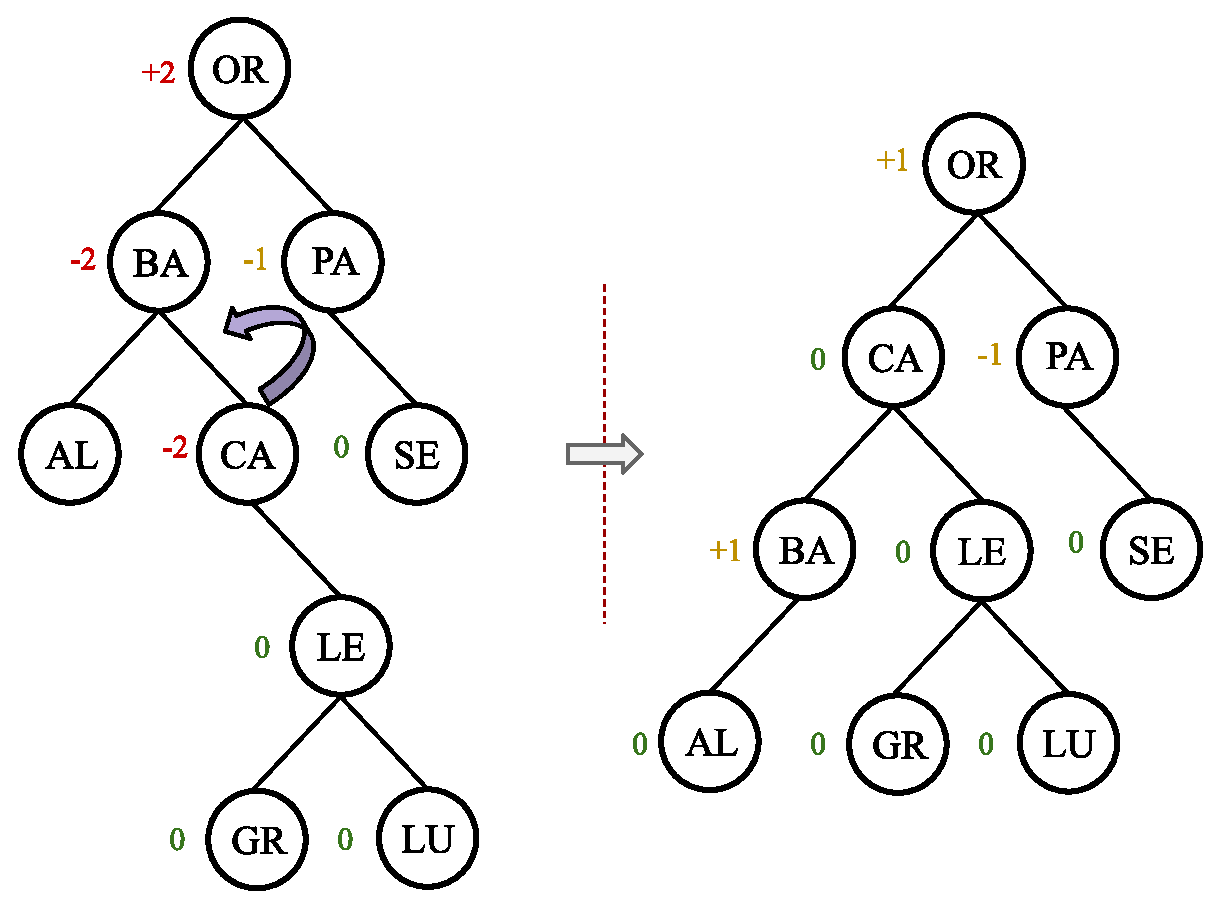
\includegraphics[width=0.6\textwidth]{images/AVLInsertion6.eps}
  \end{center}
  \caption{Representación en forma de árbol del ejemplo de código en HTML.}
  \label{fig:AVLInsertion6}
\end{figure}
